\documentclass[11pt,fontset=fandol]{ctexart}

\usepackage[a4paper,margin=1in]{geometry}
\usepackage{amsmath,amsfonts,amssymb}
\usepackage{graphicx}
\usepackage{enumitem}
\usepackage{booktabs,longtable}
\usepackage{pdfpages}
\usepackage[hidelinks]{hyperref}
\usepackage{xurl}
\usepackage{verbatim}
\setlength{\emergencystretch}{8em}

\title{$k=1$（最近邻，$K=2$）lazy 环 + 单向 shortcut：\\非捷径节点等概率（原地/左右各 $1/3$）基准下的双峰最小示例\\（Chebyshev 解析生成函数 + AW 反演；flux 交叉验证）}
\author{}
\date{}

\setlist[itemize]{itemsep=0pt,topsep=4pt,parsep=0pt,partopsep=0pt}

\begin{document}
\sloppy
\maketitle

\section{模型（最简单情形：$k=1$ / $K=2$）}
节点为 $0,1,\dots,N-1$ 的环。设 $0<q<1$，lazy 最近邻随机游走的转移为
\[
P(i\to i)=1-q,\qquad P(i\to i\pm1)=\frac{q}{2}\quad(\mathrm{mod}\ N).
\]
若希望 ``原地/左右等概率''，取
\[
1-q=\frac{q}{2}=\frac{1}{3}\quad\Longleftrightarrow\quad q=\frac{2}{3}.
\]
加入单条有向 shortcut $u\to v$，采用 ``从 self-loop 拿走概率'' 的模型：
\[
P(u\to u)=1-q-p,\qquad P(u\to v)=p,\qquad 0\le p\le 1-q.
\]
因此在等概率基准下，$p$ 可以理解为：在特殊点 $u$ 处，以概率 $p$ 执行一次额外的有向跳转 $u\to v$（并相应减少 ``原地'' 的概率）。
注意：这里的 ``等概率'' 指的是\textbf{非捷径节点}的三选一（原地/左右各 $1/3$，即 $q=2/3$），并不意味着在加入 shortcut 后源点 $u$ 的四个动作等概率；
若采用 ``原地/左右/捷径'' 四个动作在 $u$ 处各 $1/4$ 的规则，见第 \ref{sec:equal4} 节（equal4）。
目标点 $\mathrm{target}$ 为吸收态，研究从起点 $n_0$ 到 $\mathrm{target}$ 的首达时间 $T$ 的 pmf
\[
f(t)=\Pr(T=t),\qquad t=1,2,\dots
\]
是否出现双峰。

\section{数值方法（flux）与解析方法（AW 反演）}
\paragraph{解析生成函数（lazy 情况是否变化？）}
lazy 情况的解析公式\textbf{不会另起一套推导}，而是通过 $q\in(0,1)$ 直接进入谱结构：
缺陷自由的特征值为 $\lambda_k=1-q+q\cos(2\pi k/N)$。
完整的解析生成函数（含 directed shortcut，且 $p$ 从 self-loop 挪出）已经在
\texttt{deriv\_k2/note\_k2.pdf} 中给出（对应 \texttt{.tex} 里的
$\tilde Q(d,z)$、$\tilde S_{n_0}(n,z)$ 与 $\tilde F_{n_0\to n}(z)$ 的 Chebyshev 闭式）。

\paragraph{AW 反演（从 $\tilde F(z)$ 得到 $f(t)$）}
给定 $\tilde F(z)=\sum_{t\ge0} f(t)z^t$，用离散圆周采样做 Cauchy 系数反演：
取 $z_k=r e^{2\pi i k/m}$，则
\[
f(t)\approx r^{-t}\frac{1}{m}\sum_{k=0}^{m-1}\tilde F(z_k)\,e^{-2\pi i k t/m},
\qquad t=1,2,\dots
\]
实现上用 FFT 得到整段系数。本报告对应实现为 \texttt{lazy\_ring\_aw\_chebyshev.py}。

\paragraph{flux（时域推进）用于交叉验证}
将 $\mathrm{target}$ 设为吸收态并推进未吸收分布 $p_t(i)$。
每步后强制 $p_t(\mathrm{target})=0$；每步首达概率是流入吸收态的 flux：
\[
f(t+1)=\sum_{i\neq \mathrm{target}} p_t(i)\,P(i\to \mathrm{target}).
\]
本报告对应实现为 \texttt{lazy\_ring\_flux\_bimodality.py}（不建 $(N\times N)$ 矩阵，逐步推进并记录 flux）。

\section{双峰判据（paper 风格 + 宏观分离）}\label{sec:criterion}
对离散 pmf，曲线在小 $t$ 处常出现 ``锯齿/起伏''（尤其是最近邻模型），因此本报告使用严格局部峰并加阈值：
\begin{itemize}
  \item \textbf{严格局部峰：}若 $f(t)>f(t-1)$ 且 $f(t)>f(t+1)$ 且 $f(t)\ge h_{\min}$，则称 $t$ 为峰。
  \item \textbf{双峰（paper）：}存在至少两个峰，并要求第二高峰高度 $\ge 1\%$ 的最高峰高度。
  \item \textbf{宏观双峰（可选）：}在 paper 双峰基础上，再要求两最高峰满足 $t_2/t_1\ge 10$（强调时间尺度分离）。
\end{itemize}

\section{主要结论}
在本文设定的 $k=1$（$K=2$）lazy 环 + 单向 shortcut 模型下，得到如下可复现结论（AW 解析反演，并用 flux 交叉验证）：
\begin{itemize}
  \item \textbf{selfloop（从自环挪出 $p$）在小 $p$ 下可出现双峰：}最小示例 $N=10,q=2/3,u=n_0=1\to v=\mathrm{target}=5,p=0.006666\ldots$ 在 $h_{\min}=10^{-7}$ 下有两处严格局部峰（见第 \ref{sec:min-selfloop} 节与图 \autoref{fig:n10-example-cn}），且 $N=11$（奇数）下同样成立（图 \autoref{fig:n11-example-cn}）。
  \item \textbf{小 $N$ 全扫描显示宏观双峰从 $N=10$ 起出现：}在等概率基准 $q=2/3$、$\beta=0.02$ 且 $u=n_0\to v=\mathrm{target}$ 的设定下，对 $N=3..60$ 扫描所有终点，宏观双峰主要出现在距离较大的终点（见热图与附录全表）。
  \item \textbf{equal4（源点四动作各 $1/4$）在 paper-like 几何下无双峰：}对 $N=10..200$ 扫描（paper-like：$u=n_0+5, v=\mathrm{target}+1$），paper/macro 双峰计数均为 0（见第 \ref{sec:equal4} 节）。
  \item \textbf{shortcut 强度增大将抑制双峰：}在 paper-like 几何 $N=100,u=6\to v=51$ 下，$\beta$ 扫描显示当 $\beta\gtrsim 0.07$（$p=\beta(1-q)$）时双峰判据不再成立（见表 \autoref{tab:selfloop-beta-scan-cn} 与图 \autoref{fig:selfloop-beta-sens-cn}）。
\end{itemize}

\section{最小示例：$N=10$（selfloop 模型；非 equal4）}\label{sec:min-selfloop}
为尽量 ``从小 $N$ 开始''，这里选取一个 $N=10$ 的最小示例；并刻意挑选一个 \textbf{严格局部峰数目就是 2} 的案例来避免 ``多峰起伏'' 的误读。

参数为：
\begin{itemize}
  \item $N=10$，$q=2/3$（原地/左右各 $1/3$）；
  \item $n_0=1$，$\mathrm{target}=5$；
  \item shortcut（selfloop 规则，\textbf{非等概率 1/4}）：$u=n_0=1\to v=\mathrm{target}=5$，$p=0.006666\ldots$（例如取 $\beta=0.02$ 使 $p=\beta(1-q)=0.02/3$）；
  \item 计算：推进到生存概率小于 $10^{-14}$（尾部剩余质量上界）。
\end{itemize}

该例在阈值 $h_{\min}=10^{-7}$ 下只有两处严格局部峰，峰时间为 $t_1=1,t_2=10$，并满足 $t_2/t_1=10$ 的宏观分离要求。

\begin{figure}[!htbp]
  \centering
  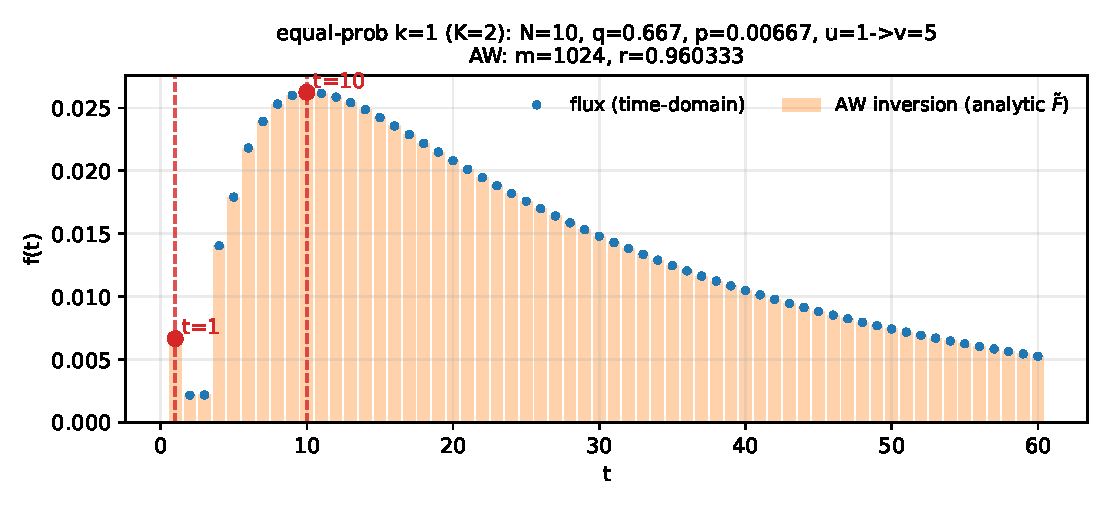
\includegraphics[width=0.92\linewidth]{figures/lazy_ring_flux_bimodality/lazy_K2_equalprob_N10_aw_vs_flux.pdf}
  \caption{$k=1$（$K=2$）lazy 环 + 单向 shortcut 的首达 pmf：$N=10,q=2/3,p=0.006666\ldots,u=1\to v=5$。
  AW 反演（解析 $\tilde F$）与 flux（时域推进）叠加对比，二者一致；标注两峰时间 $t_1=1,t_2=10$。}
  \label{fig:n10-example-cn}
\end{figure}

\section{奇偶 $N$ 示例：$N=11$（奇数）同样双峰}
为考察奇偶性，这里再给出一个 $N=11$（奇数）示例，在同样的等概率基准 $q=2/3$ 与同样的 shortcut 设定
（$u=n_0=1\to v=\mathrm{target}=5$，$p=0.006666\ldots$）下，
在阈值 $h_{\min}=10^{-7}$ 时同样只有两处严格局部峰，峰时间为 $t_1=1,t_2=10$。
\begin{figure}[!htbp]
  \centering
  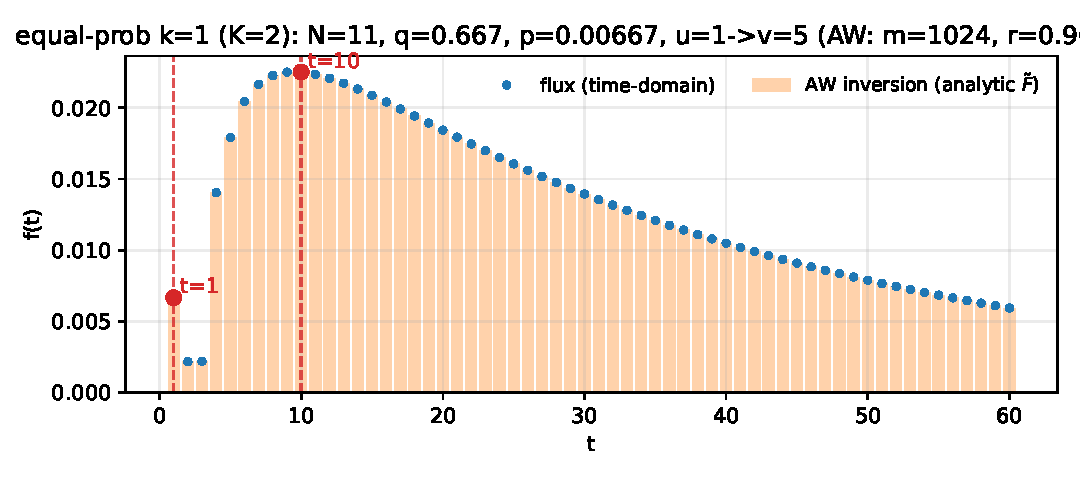
\includegraphics[width=0.92\linewidth]{figures/lazy_ring_flux_bimodality/lazy_K2_equalprob_N11_target5_aw_vs_flux.pdf}
  \caption{$N=11$（奇数）下的首达 pmf（其余参数同上）。AW 与 flux 完全重合；标注两峰时间 $t_1=1,t_2=10$。}
  \label{fig:n11-example-cn}
\end{figure}

\section{小 $N$ 扫描（AW 解析）：哪些终点会出现宏观双峰？}
固定等概率基准 $q=2/3$、$n_0=1$，并取最简单的 shortcut：$u=n_0\to v=\mathrm{target}$，
并固定 $\beta=0.02$（即 $p=\beta(1-q)=0.006666\ldots$），对 $N=3..60$ 扫描所有终点（除 $n_0$ 以外）。

\paragraph{扫描方法}
对每个 $N$ 与每个 $\mathrm{target}\neq n_0$：
\begin{itemize}
  \item 用 \texttt{lazy\_ring\_aw\_chebyshev.py} 中的 Chebyshev 闭式生成函数 $\tilde F(z)$；
  \item 用离散 Cauchy/AW 反演得到 $f(t)$，取 $t_{\max}=\lceil 4N^2\rceil$；
  \item AW 参数取 $m=\mathrm{pow2}(\mathrm{oversample}\cdot(t_{\max}+1))$（默认 \texttt{oversample=4}），并选 $r$ 使 $r^m=10^{-18}$；
  \item 对 $f(t)$ 做严格局部峰检测（阈值 $h_{\min}=10^{-7}$），并计算 paper/macro 判据与两主峰时间 $(t_1,t_2)$。
\end{itemize}
扫描结果的完整数据表（包含每个 $N$ 的每个终点）放在附录表 \ref{tab:fullscan-cn}。

\paragraph{扫描可视化（热图）}
使用第 \ref{sec:criterion} 节的 ``宏观双峰'' 判据（$h_{\min}=10^{-7}$，第二峰 $\ge 1\%$，且 $t_2/t_1\ge 10$），
将满足宏观双峰的点以后峰时间 $t_2$ 着色：
横轴为环距离 $d=\mathrm{dist}(n_0,\mathrm{target})$，纵轴为 $N$（空白表示未满足宏观双峰）。
\begin{figure}[!htbp]
  \centering
  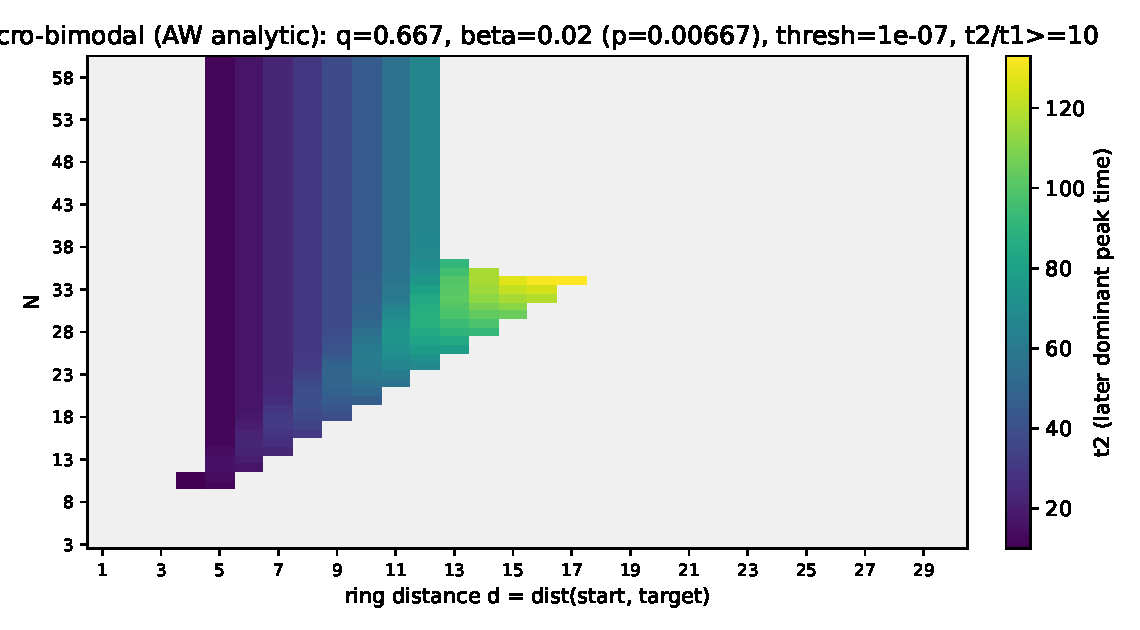
\includegraphics[width=0.92\linewidth]{figures/lazy_ring_flux_bimodality/lazy_K2_equalprob_macro_scan_N3_60.pdf}
  \caption{全扫描热图（AW 解析反演）：$N=3..60$、距离 $d$ 与宏观双峰的对应关系。图中颜色为后峰时间 $t_2$。}
\end{figure}
\noindent
该扫描显示：在本设定下，宏观双峰从 $N=10$ 开始出现，且主要出现在距离较大的终点（例如接近对径点）。
当 $N$ 继续增大时，pmf 往往会出现额外的 ``微结构'' 局部峰（这是离散时间首达分布的真实起伏），
因此报告中区分了 ``paper 双峰''（至少两峰）与 ``宏观双峰''（两主峰时间尺度分离）。

\section{“等概率走捷径”规则：在 $u$ 处四个动作各 $1/4$（equal4）}\label{sec:equal4}
前面的解析推导（\texttt{deriv\_k2/note\_k2.pdf}）对应的是 ``从 $u$ 的 self-loop 挪出概率 $p$ 到 $u\to v$''：
$P(u\to u)=1-q-p$、$P(u\to u\pm1)=q/2$ 不变。

若采用 ``走捷径的概率与其他动作等概率'' 的规则，则在 shortcut 源点 $u$ 处应改成四个动作均匀：
\[
P(u\to u)=P(u\to u\pm1)=P(u\to v)=\frac14.
\]
这会同时改变 $u\to u\pm1$ 的概率（不再保持 $q/2$），因此 \textbf{解析生成函数形式会随之改变}。
不过该缺陷仍然只修改了转移矩阵的 \textbf{一列（从 $u$ 出发的出边）}，可以用 Sherman--Morrison 的 rank-1 更新得到
$\tilde S(z)=(I-zA)^{-1}$ 并由
$\tilde F_{n_0\to n}(z)=\tilde S_{n_0}(n,z)/\tilde S_{n}(n,z)$ 得到首达生成函数。
本报告的实现为 \texttt{lazy\_ring\_aw\_chebyshev.py} 中的 \texttt{fpt\_pmf\_aw\_equal4}，并用 flux 交叉验证。

\paragraph{结论（paper-like 几何下无双峰）}
在本文采用的 paper-like 几何（$n_0=1$，$\mathrm{target}=\lfloor N/2\rfloor$，$u=n_0+5$，$v=\mathrm{target}+1$）下，
对 $N=10..200$ 扫描，\textbf{equal4 规则下 paper/macro 双峰均为 0}（阈值 $h_{\min}=10^{-7}$，第二峰 $\ge 1\%$，宏观分离 $t_2/t_1\ge 10$）。
代表性结果见表 \autoref{tab:equal4-paper-geom-cn}，$N=100$ 的曲线对比如图 \autoref{fig:paper-geom-equal4-compare}：
同一几何下，selfloop 小 $p$ 模型出现两主峰，而 equal4 规则变为单峰。
\begin{table}[!htbp]
\centering
\small
\begin{tabular}{rrrrrr}
\toprule
$N$ & $u$ & $v$ & paper & macro & $t_\mathrm{peak}$\\
\midrule
20 & 6 & 11 & 0 & 0 & 34\\
50 & 6 & 26 & 0 & 0 & 27\\
100 & 6 & 51 & 0 & 0 & 27\\
160 & 6 & 81 & 0 & 0 & 27\\
200 & 6 & 101 & 0 & 0 & 27\\
\bottomrule
\end{tabular}
\caption{equal4 概率规则下（在 $u$ 处四个动作各 $1/4$），采用 paper-like 几何 $n_0=1$, $\mathrm{target}=\lfloor N/2\rfloor$, $u=n_0+5$, $v=\mathrm{target}+1$ 的代表性结果。}
\label{tab:equal4-paper-geom-cn}
\end{table}

\begin{figure}[!htbp]
  \centering
  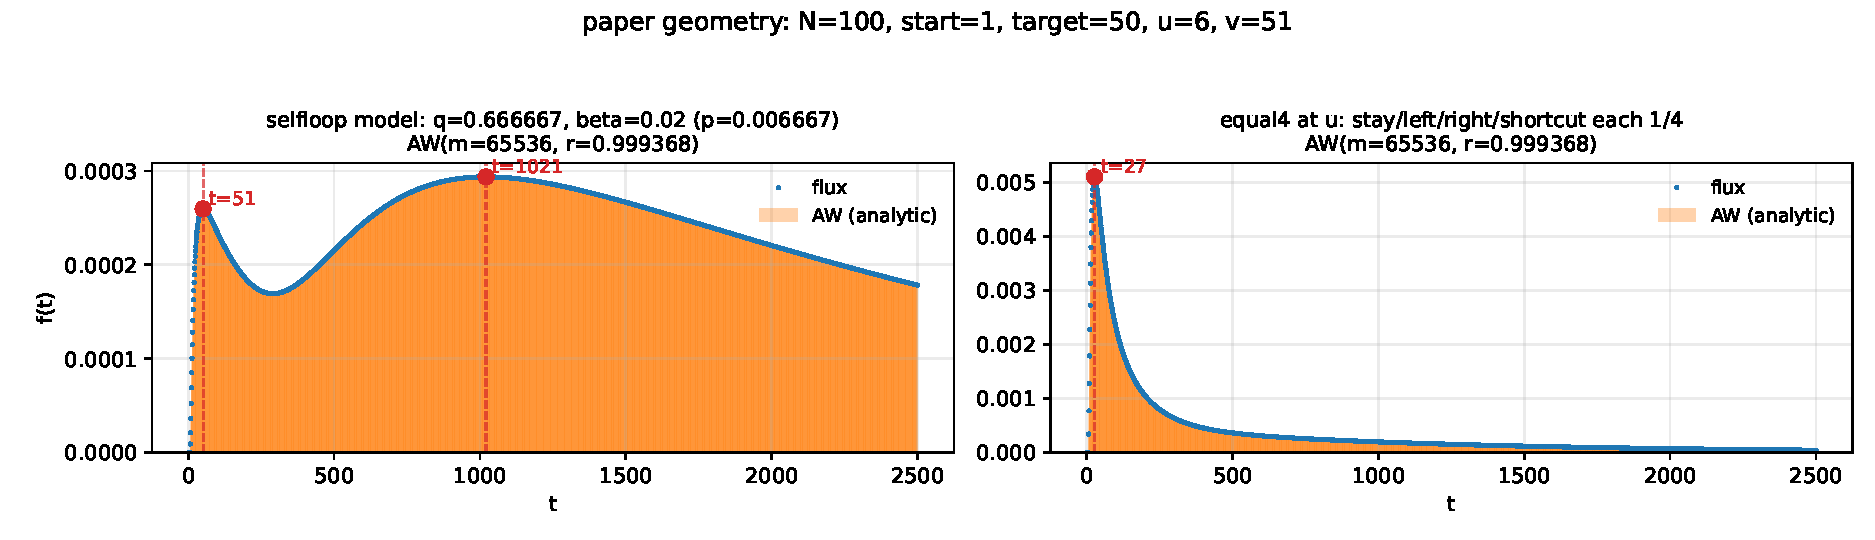
\includegraphics[width=0.98\linewidth]{figures/lazy_ring_flux_bimodality/lazy_K2_paper_geometry_selfloop_vs_equal4_N100.pdf}
  \caption{paper-like 几何（$N=100$，$u=6\to v=51$）下，两种概率规则对比：左为 selfloop（$p=\beta(1-q),\beta=0.02$）出现两主峰；右为 equal4（在 $u$ 处四个动作各 $1/4$）为单峰。AW 反演与 flux 叠加一致。}
  \label{fig:paper-geom-equal4-compare}
\end{figure}

\subsection{为什么 $p$ 大时更不容易双峰？（selfloop 的 $\beta$ 扫描）}
直观机制是：selfloop 模型下 $p$ 越大，越容易在到达 $\mathrm{target}$ 之前先走上 shortcut，从而把到达时间集中到一个更早的时间尺度；
这会使得 ``慢尺度'' 的扩散到达峰被压低甚至消失（从而不再满足双峰判据）。
下面以 paper-like 几何（$N=100,u=6\to v=51$）为例，扫描 $\beta$（$p=\beta(1-q)$）得到：
当 $\beta\gtrsim 0.07$（即 $p\gtrsim 0.023$）时，paper/macro 双峰不再成立（见表 \autoref{tab:selfloop-beta-scan-cn}），并且曲线形状也从双峰变为单峰（见图 \autoref{fig:selfloop-beta-sens-cn}）。

\begin{table}[!htbp]
\centering
\small
\begin{tabular}{rrrrrr}
\toprule
$\beta$ & $p$ & paper & macro & $t_1$ & $t_2$\\
\midrule
0 & 0 & 0 & 0 & -- & --\\
0.0005 & 0.000166667 & 1 & 1 & 54 & 1241\\
0.001 & 0.000333333 & 1 & 1 & 54 & 1234\\
0.002 & 0.000666667 & 1 & 1 & 54 & 1221\\
0.005 & 0.00166667 & 1 & 1 & 53 & 1182\\
0.01 & 0.00333333 & 1 & 1 & 53 & 1123\\
0.02 & 0.00666667 & 1 & 1 & 51 & 1021\\
0.03 & 0.01 & 1 & 1 & 50 & 934\\
0.05 & 0.0166667 & 1 & 1 & 48 & 777\\
0.07 & 0.0233333 & 0 & 0 & -- & --\\
0.1 & 0.0333333 & 0 & 0 & -- & --\\
0.15 & 0.05 & 0 & 0 & -- & --\\
0.2 & 0.0666667 & 0 & 0 & -- & --\\
0.3 & 0.1 & 0 & 0 & -- & --\\
0.5 & 0.166667 & 0 & 0 & -- & --\\
1 & 0.333333 & 0 & 0 & -- & --\\
\bottomrule
\end{tabular}
\caption{paper-like 几何（$N=100,u=6\to v=51$）下，selfloop 模型的 $\beta$ 扫描结果（$p=\beta(1-q)$）。}
\label{tab:selfloop-beta-scan-cn}
\end{table}

\begin{figure}[!htbp]
  \centering
  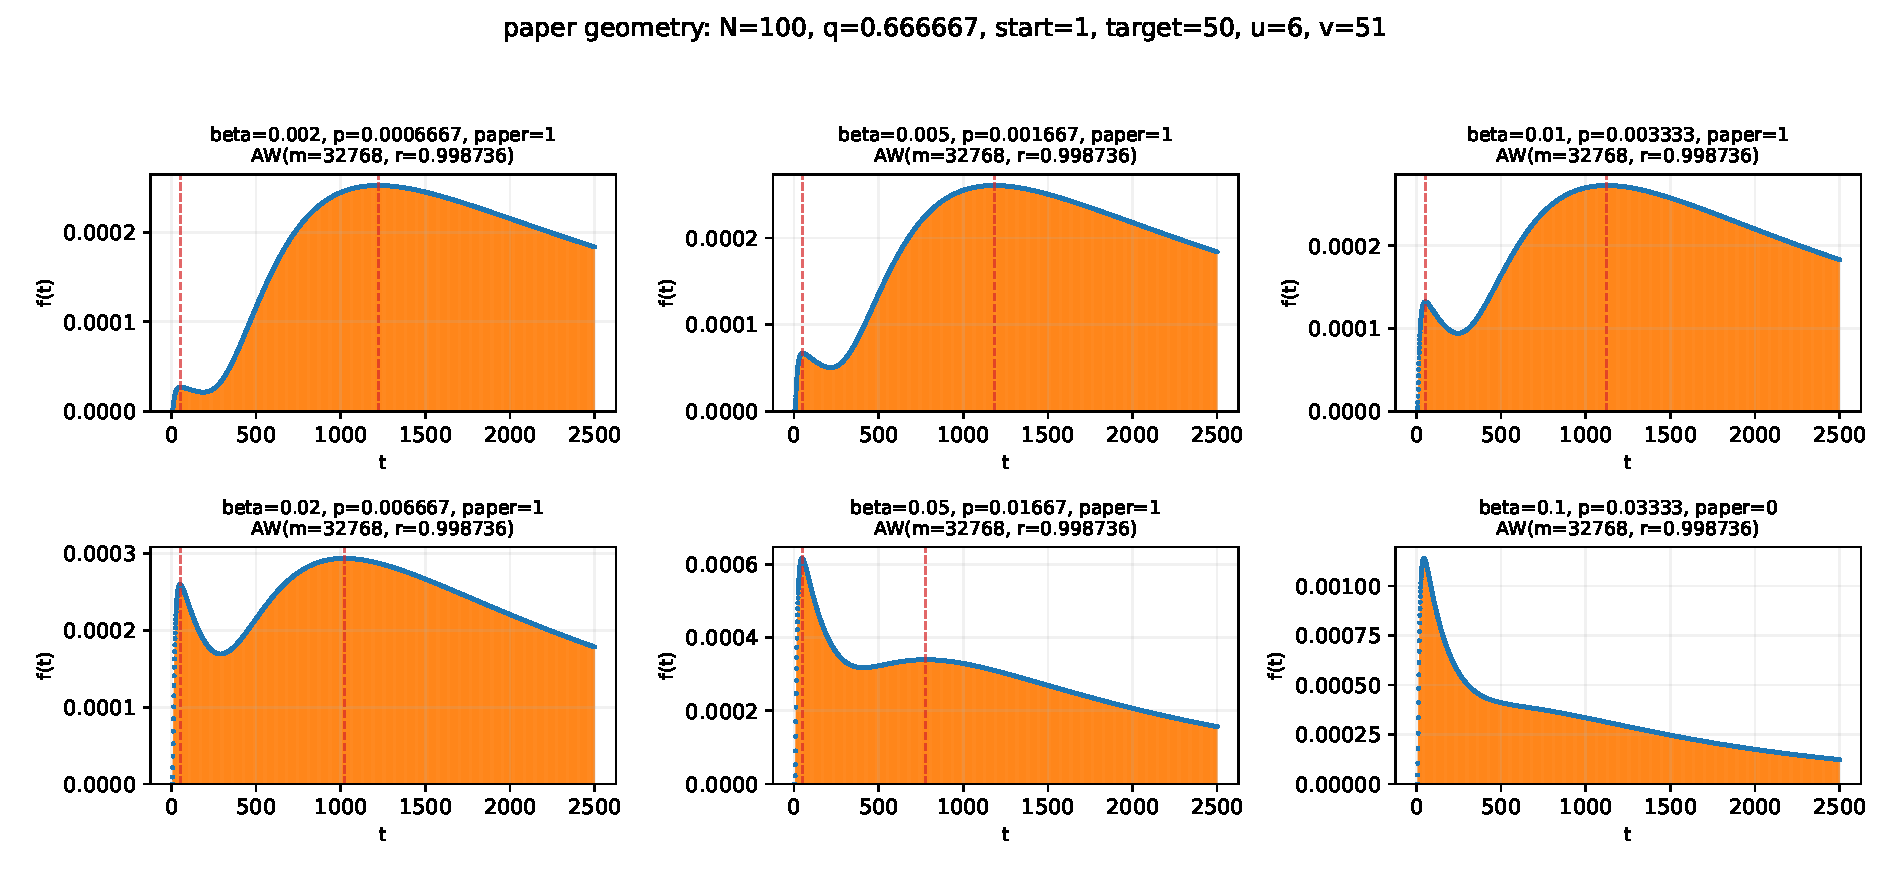
\includegraphics[width=0.98\linewidth]{figures/lazy_ring_flux_bimodality/lazy_K2_selfloop_beta_sensitivity_N100.pdf}
  \caption{selfloop 模型在 paper-like 几何（$N=100,u=6\to v=51$）下的 $\beta$ 敏感性：$p=\beta(1-q)$。
  随着 $p$ 增大，双峰逐步消失。每个子图均为 AW 反演（解析）与 flux 叠加。}
  \label{fig:selfloop-beta-sens-cn}
\end{figure}

\section{对比：\texttt{ring\_valley.tex}（非 lazy + 加边重归一）里 $K=2$ 为何“无双峰”？}
\texttt{ring\_valley.tex} 与 \texttt{valley\_study.py} 使用的是另一套（更接近原论文 Fig.~3 的）网络/概率构造：
\begin{itemize}
  \item \textbf{非 lazy：}从每个点以均匀概率跳向 $K$ 个近邻（无自环）。
  \item \textbf{shortcut 的概率分配：}在源点 $\mathrm{src}$ 处\emph{新增}一条有向边（例如 $6\to (N/2+1)$），并将源点所有出边重归一为 $1/(K+1)$（即原来的每条近邻边从 $1/K$ 降为 $1/(K+1)$）。
  \item \textbf{$K=2$ 的 parity 处理：}为了去掉周期 2 的“锯齿微峰”，先做 2 步 coarse-grain 再按 Fig.~3 规则找峰。
\end{itemize}
在这套构造下，扫描得到 $K=2$ 在相当大的 $N$ 范围内都不满足双峰判据（\texttt{ring\_valley.tex} 中也明确写出）。
我们用精确主方程推进（直到尾部剩余质量 $<10^{-14}$）复现这一点，示例如 \autoref{tab:valley-report-k2-cn}：每个 $N$ 在 coarse-grain 后都只剩 1 个主峰，因此不存在双峰。
\begin{table}[!htbp]
\centering
\begin{tabular}{rrrrr}
\toprule
$N$ & $K$ & $\mathrm{peaks}$ & $t_{\mathrm{peak}}$ & $A(t_{\mathrm{peak}})$\\
\midrule
10 & 2 & 1 & 4 & 0.0740740740741\\
20 & 2 & 1 & 12 & 0.0250960268977\\
50 & 2 & 1 & 10 & 0.0153956437253\\
100 & 2 & 1 & 10 & 0.0153956437253\\
160 & 2 & 1 & 10 & 0.0153956437253\\
\bottomrule
\end{tabular}
\caption{valley\_report 模型下 $K=2$ 的峰数（在 2 步 coarse-grain 后）示例：每个 $N$ 仅剩 1 个主峰，因此不存在双峰。}
\label{tab:valley-report-k2-cn}
\end{table}


下面给出一个更直观的对比图：\textbf{左}为 \texttt{ring\_valley.tex} 的 $K=2$ 模型（coarse-grain 后仅 1 峰），\textbf{右}为本文报告采用的 lazy selfloop 概率模型（在相同几何 shortcut：$u=6\to v=51$ 下出现两主峰）。
\begin{figure}[!htbp]
  \centering
  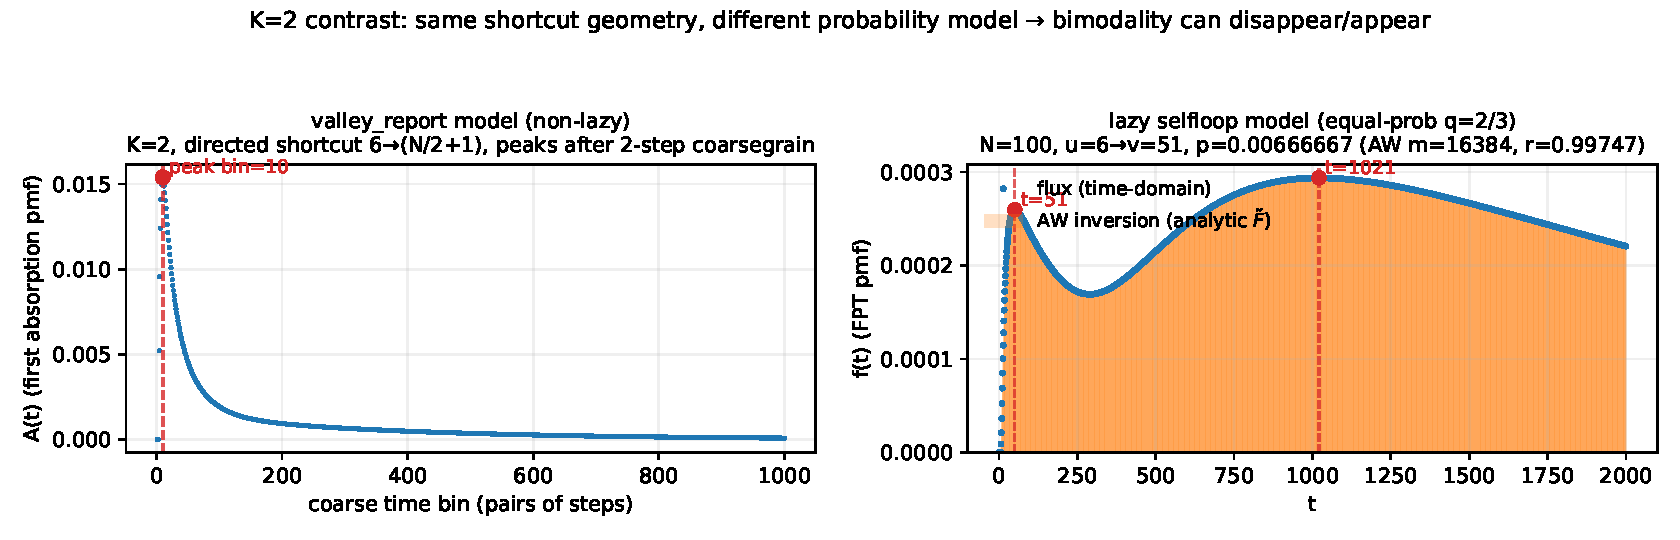
\includegraphics[width=0.96\linewidth]{figures/lazy_ring_flux_bimodality/k2_valley_report_vs_lazy_contrast.pdf}
  \caption{$K=2$ 对比：相同几何 shortcut，不同概率分配规则会导致“无双峰/有双峰”的差异。}
\end{figure}

\section{下一步建议（不在本文中实做）}
为系统性定位 ``从什么时候开始出现双峰''，一种直接做法是做参数平面扫描并记录 $(t_1,t_2)$：
\begin{itemize}
  \item \textbf{扫 $(q,p)$ 或 $(q,\beta)$：}固定几何（例如 paper-like 的 $u=n_0+5, v=\mathrm{target}+1$），对 $q\in(0,1)$ 与 $p\in[0,1-q]$（或 $p=\beta(1-q)$）网格扫描；对每个点用 AW 输出 $f(1..t_{\max})$，计算 paper/macro 与 $(t_1,t_2)$，画热图（例如 ``是否双峰''、或 ``$t_2$''）。
  \item \textbf{扫几何：}固定 $q,p$，对终点（距离 $d$）以及 $(u,v)$ 的相对位置做扫描，比较 ``固定 $u,v$'' 与 ``允许换 $u,v$'' 两种口径下双峰是否更常见。
  \item \textbf{稳健性：}为避免小 $t$ 处锯齿造成误判，可加入 valley 深度/coarse-grain（参考 \texttt{ring\_valley.tex} 的 2 步 coarse-grain）作为补充判据，并用 flux 做少量交叉验证。
\end{itemize}

\section{复现命令}
\begin{itemize}
  \item 生成该图（会写入 \texttt{figures/...}）：\path{python3 code/plot_lazy_k2_example.py}
  \item 生成奇数 $N=11$ 的对照图：\path{python3 code/plot_lazy_k2_example.py --N 11 --target 5 --v 5 --tplot 60}
  \item 生成全扫描热图（AW 解析）：\path{python3 code/plot_lazy_k2_aw_distance_scan.py --N-min 3 --N-max 60}
  \item 生成全扫描数据表（CSV + 附录 longtable）：\path{python3 code/scan_lazy_k2_aw_fulltable.py --N-min 3 --N-max 60}
  \item 生成对径终点多图（AW 解析，even\_small）：\path{python3 code/plot_lazy_k2_aw_antipodal_panels.py --group even_small}
  \item 生成对径终点多图（AW 解析，odd\_small）：\path{python3 code/plot_lazy_k2_aw_antipodal_panels.py --group odd_small}
  \item 生成对径终点多图（AW 解析，even\_medium）：\path{python3 code/plot_lazy_k2_aw_antipodal_panels.py --group even_medium}
  \item equal4（paper-like 几何）扫描：\path{python3 code/scan_lazy_k2_equal4_paper_geometry.py --N-min 10 --N-max 200}
  \item paper-like 几何 selfloop vs equal4 对比图：\path{python3 code/plot_lazy_k2_paper_geometry_equal4_compare.py --N 100}
  \item small-$p$ 双峰曲线集合（compact 多子图）：\path{python3 code/plot_lazy_k2_selfloop_smallp_gallery_compact.py --q 0.6666666667 --beta 0.02 --tplot 5000}
  \item 单次运行输出（含 \texttt{top2}）：\path{python3 code/lazy_ring_flux_bimodality.py --N 10 --q 0.6666667 --start 1 --target 5 --model selfloop --u 1 --v 5 --p 0.0066667 --Tmax 200000 --eps-surv 1e-14}
\end{itemize}

\appendix
\section{small-$p$ 双峰曲线集合（selfloop；paper-like 几何）}
本附录将 selfloop 模型在 paper-like 几何、$\beta=0.02$（$p=0.006666\ldots$）下的一组双峰曲线整理为 compact 多子图（每页包含多个 $N$ 的子图）。
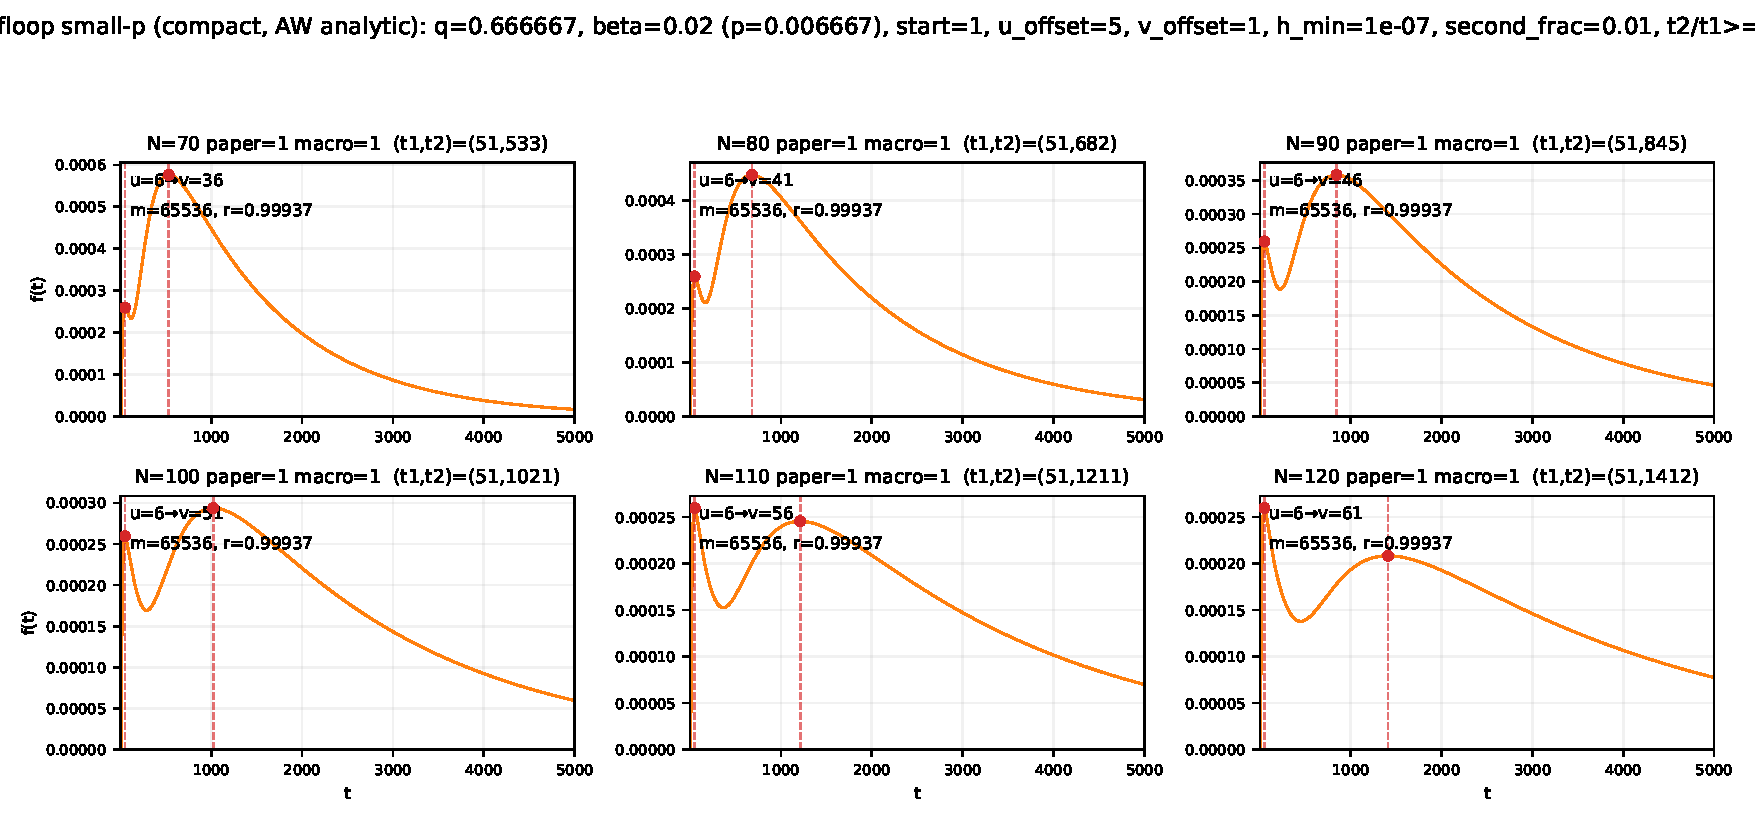
\includepdf[pages=-]{figures/lazy_ring_flux_bimodality/lazy_K2_selfloop_smallp_gallery_compact_beta0.02.pdf}

\section{补充图：对径终点 AW 曲线（多图）}
下面给出一些 ``对径终点'' 的 AW 曲线（每个子图取 $\mathrm{target}=n_0+\lfloor N/2\rfloor$），用于直观看到从小 $N$ 到较大 $N$ 的形状变化：
\begin{figure}[!htbp]
  \centering
  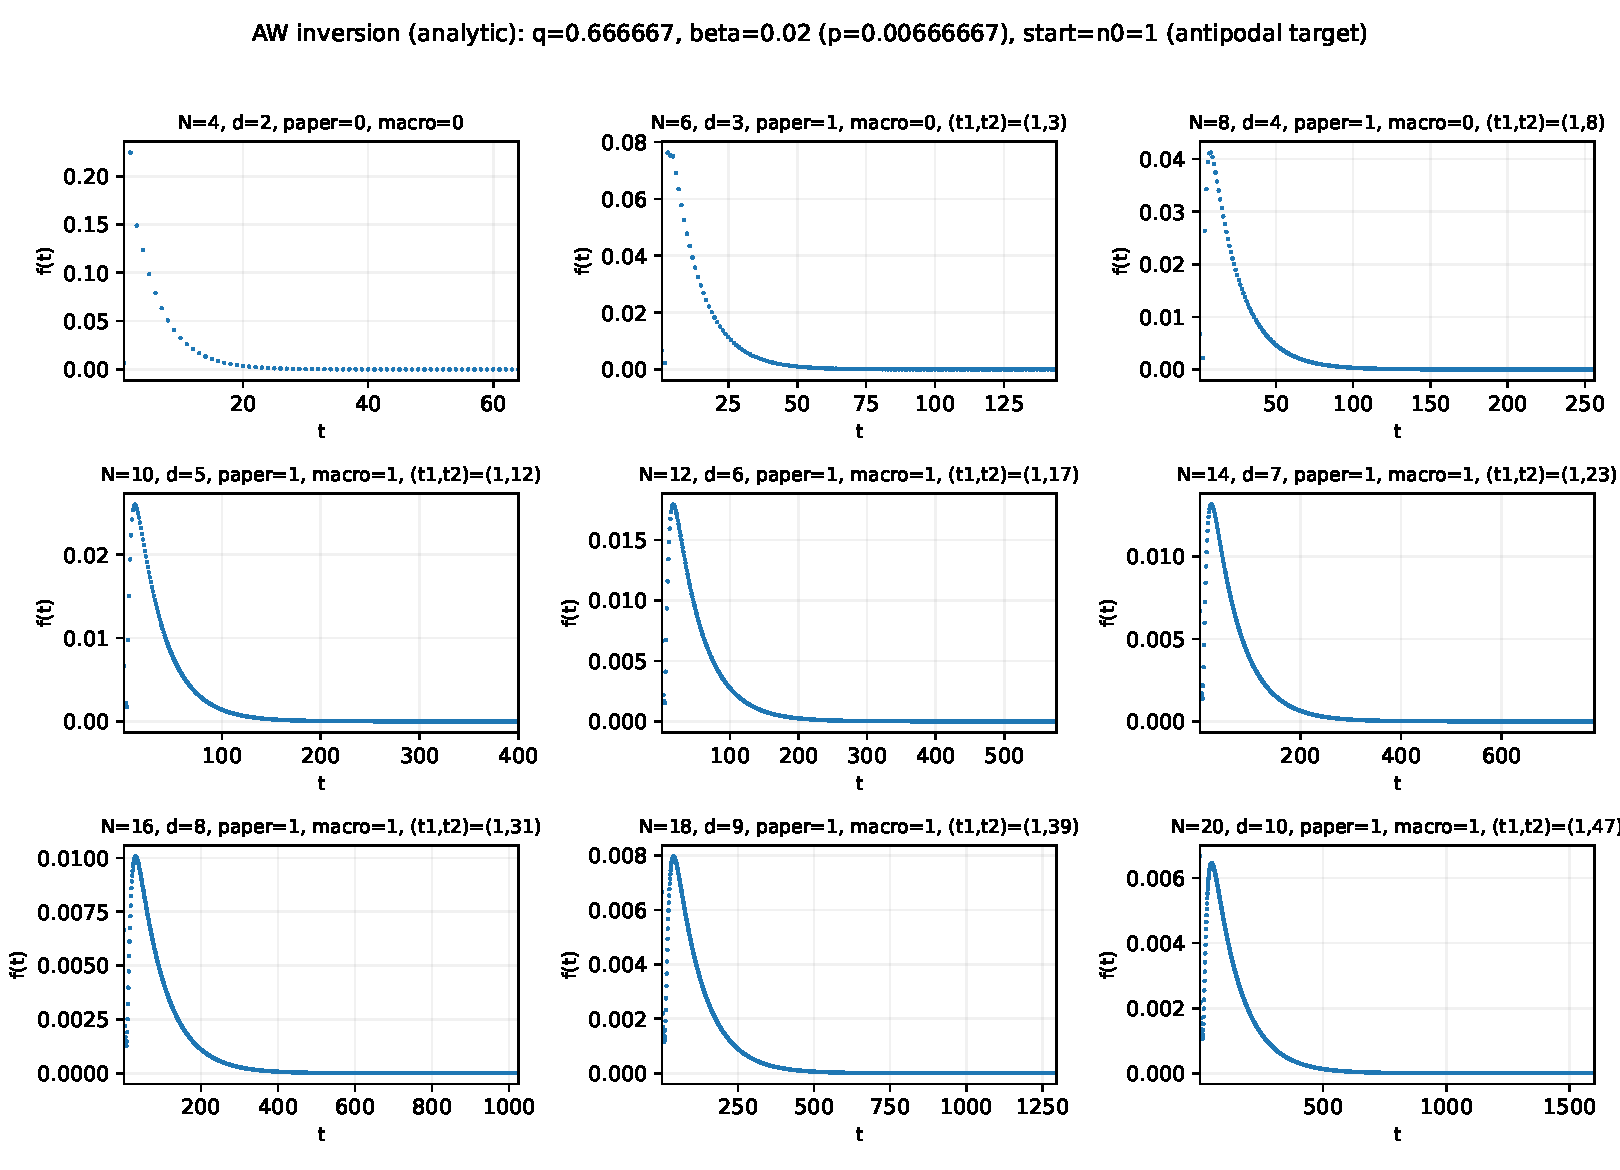
\includegraphics[width=0.92\linewidth]{figures/lazy_ring_flux_bimodality/lazy_K2_aw_antipodal_even_small.pdf}
  \caption{对径终点示例（偶数小 $N$：$N=4,6,\dots,20$）。每个子图标题标注 paper/macro 与 $(t_1,t_2)$。}
\end{figure}
\begin{figure}[!htbp]
  \centering
  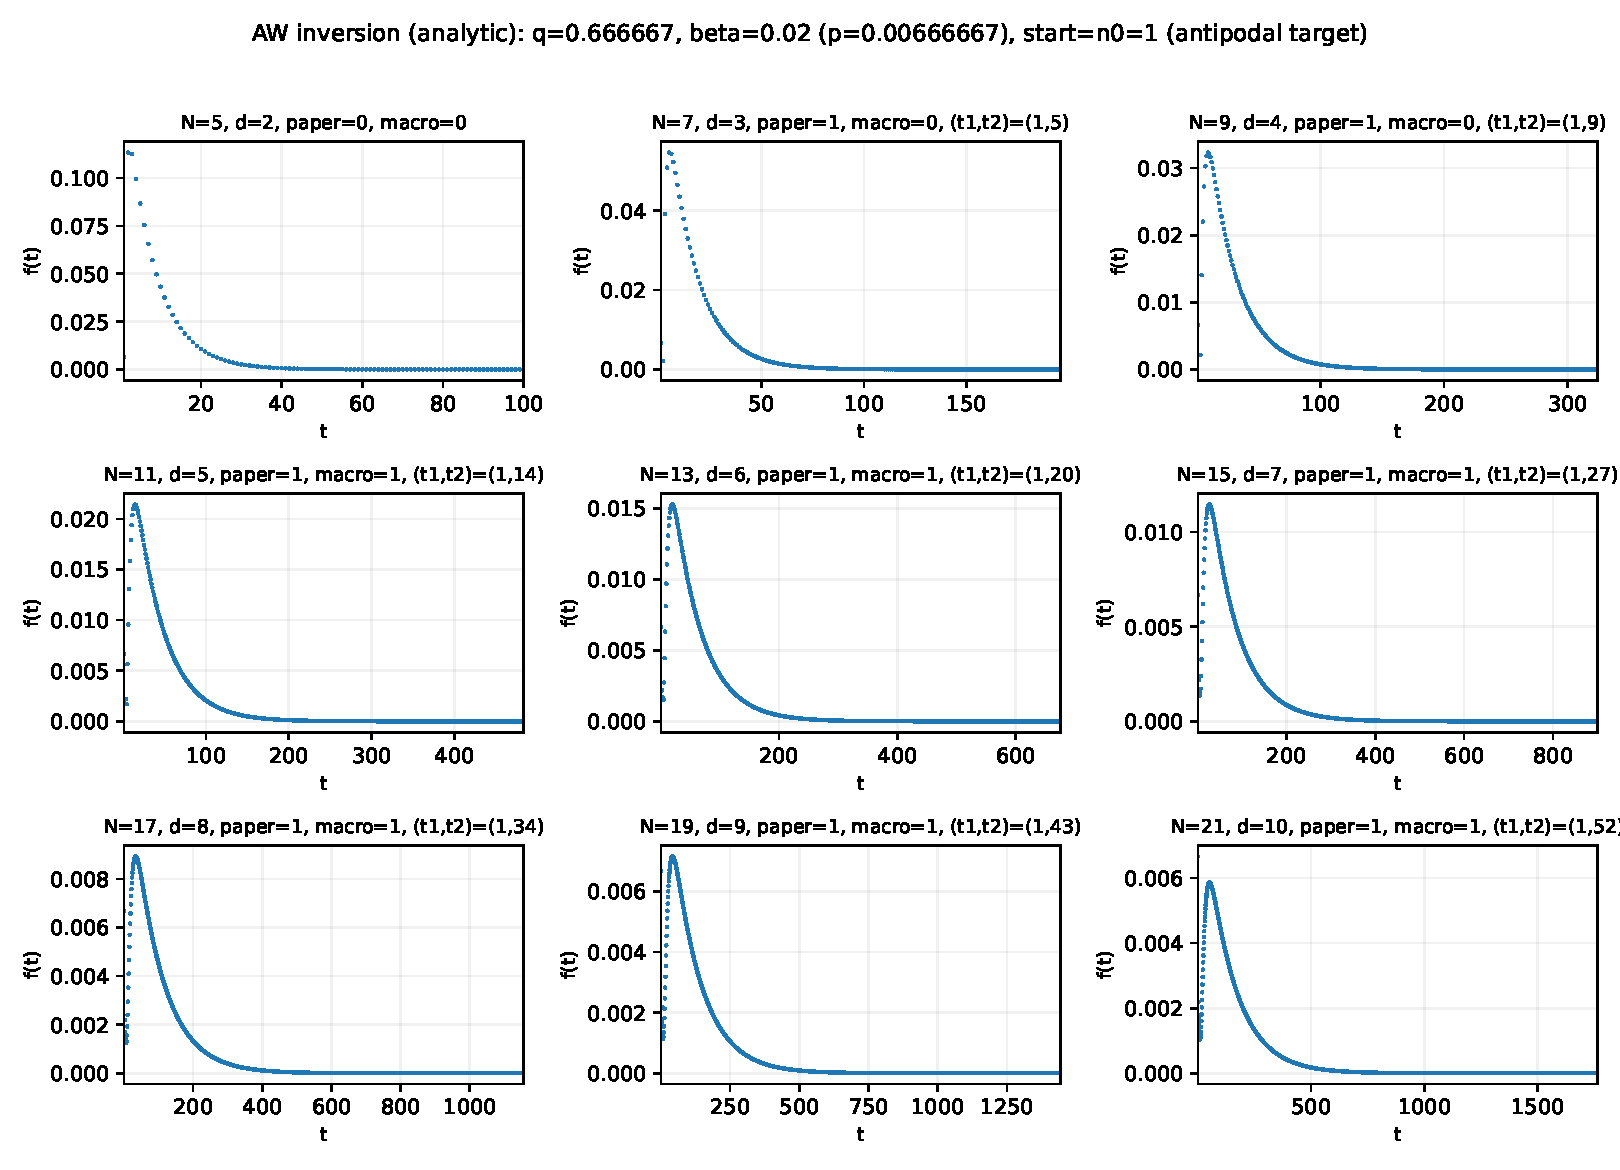
\includegraphics[width=0.92\linewidth]{figures/lazy_ring_flux_bimodality/lazy_K2_aw_antipodal_odd_small.pdf}
  \caption{对径终点示例（奇数小 $N$：$N=5,7,\dots,21$）。}
\end{figure}
\begin{figure}[!htbp]
  \centering
  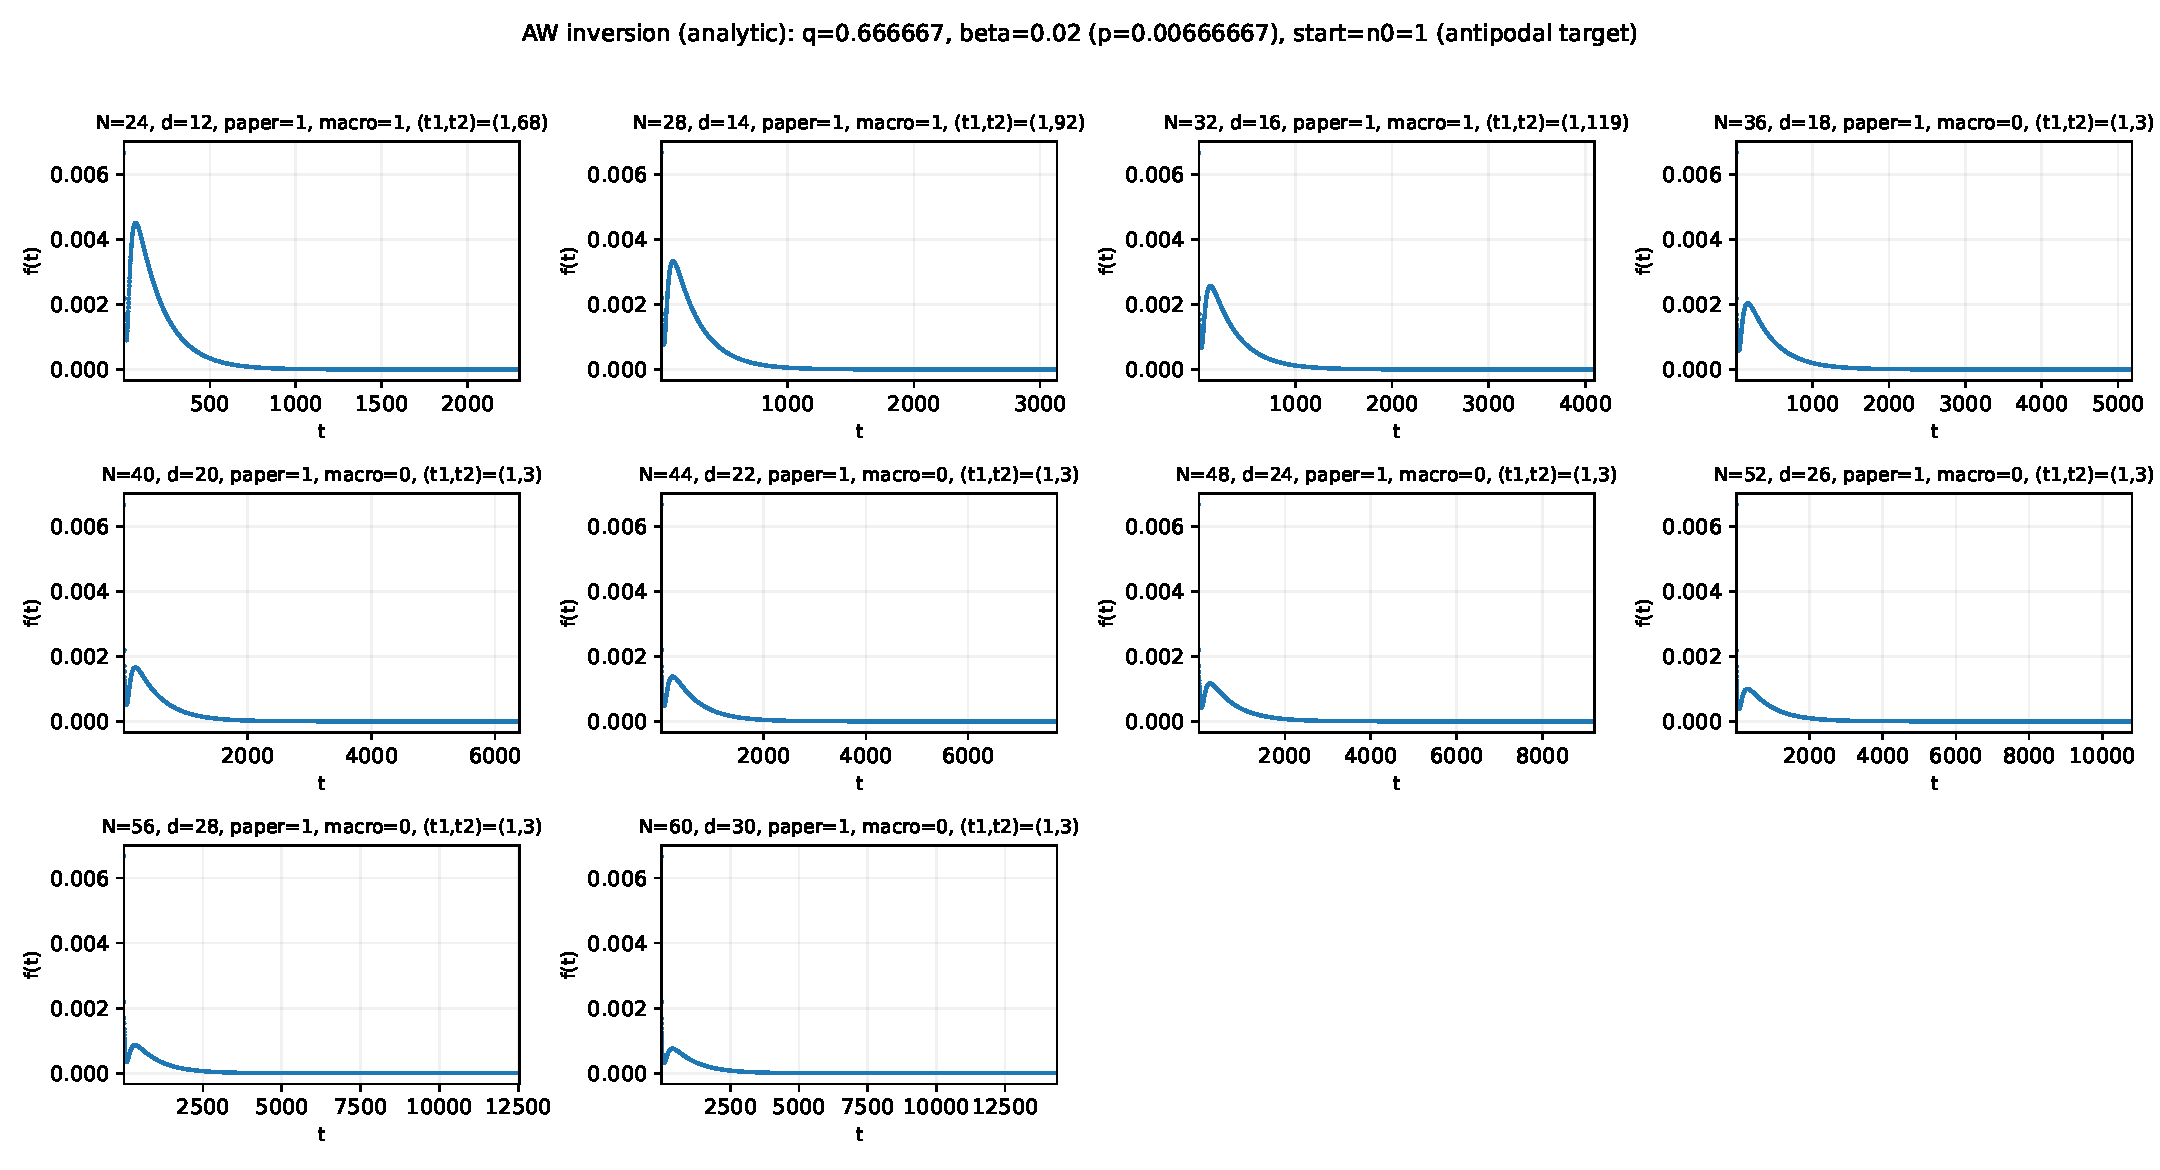
\includegraphics[width=0.92\linewidth]{figures/lazy_ring_flux_bimodality/lazy_K2_aw_antipodal_even_medium.pdf}
  \caption{对径终点示例（偶数较大 $N$：$N=24,28,\dots,60$）。}
\end{figure}

\section{全扫描数据表}
\scriptsize
\begin{longtable}{rrrrrrr}
\caption{完整扫描表（等概率基准 $q=2/3$，取 $\beta=0.02$ 使 $p=0.006666\ldots$，起点 $n_0=1$，shortcut 取 $u=n_0\to v=\mathrm{target}$）。paper/macro 为 0/1；$d$ 为 $n_0$ 到终点的环距离。}\\
\label{tab:fullscan-cn}\\
\toprule
$N$ & target & $d$ & paper & macro & $t_1$ & $t_2$\\
\midrule
\endfirsthead
\toprule
$N$ & target & $d$ & paper & macro & $t_1$ & $t_2$\\
\midrule
\endhead
\bottomrule
\endfoot
3 & 0 & 1 & 0 & 0 & -- & --\\
3 & 2 & 1 & 0 & 0 & -- & --\\
4 & 0 & 1 & 1 & 0 & 1 & 3\\
4 & 2 & 1 & 1 & 0 & 1 & 3\\
4 & 3 & 2 & 0 & 0 & -- & --\\
5 & 0 & 1 & 0 & 0 & -- & --\\
5 & 2 & 1 & 0 & 0 & -- & --\\
5 & 3 & 2 & 0 & 0 & -- & --\\
5 & 4 & 2 & 0 & 0 & -- & --\\
6 & 0 & 1 & 0 & 0 & -- & --\\
6 & 2 & 1 & 0 & 0 & -- & --\\
6 & 3 & 2 & 0 & 0 & -- & --\\
6 & 5 & 2 & 0 & 0 & -- & --\\
6 & 4 & 3 & 1 & 0 & 1 & 3\\
7 & 0 & 1 & 0 & 0 & -- & --\\
7 & 2 & 1 & 0 & 0 & -- & --\\
7 & 3 & 2 & 0 & 0 & -- & --\\
7 & 6 & 2 & 0 & 0 & -- & --\\
7 & 4 & 3 & 1 & 0 & 1 & 5\\
7 & 5 & 3 & 1 & 0 & 1 & 5\\
8 & 0 & 1 & 0 & 0 & -- & --\\
8 & 2 & 1 & 0 & 0 & -- & --\\
8 & 3 & 2 & 0 & 0 & -- & --\\
8 & 7 & 2 & 0 & 0 & -- & --\\
8 & 4 & 3 & 1 & 0 & 3 & 5\\
8 & 6 & 3 & 1 & 0 & 3 & 5\\
8 & 5 & 4 & 1 & 0 & 1 & 8\\
9 & 0 & 1 & 0 & 0 & -- & --\\
9 & 2 & 1 & 0 & 0 & -- & --\\
9 & 3 & 2 & 0 & 0 & -- & --\\
9 & 8 & 2 & 0 & 0 & -- & --\\
9 & 4 & 3 & 1 & 0 & 1 & 3\\
9 & 7 & 3 & 1 & 0 & 1 & 3\\
9 & 5 & 4 & 1 & 0 & 1 & 9\\
9 & 6 & 4 & 1 & 0 & 1 & 9\\
10 & 0 & 1 & 0 & 0 & -- & --\\
10 & 2 & 1 & 0 & 0 & -- & --\\
10 & 3 & 2 & 0 & 0 & -- & --\\
10 & 9 & 2 & 0 & 0 & -- & --\\
10 & 4 & 3 & 1 & 0 & 1 & 3\\
10 & 8 & 3 & 1 & 0 & 1 & 3\\
10 & 5 & 4 & 1 & 1 & 1 & 10\\
10 & 7 & 4 & 1 & 1 & 1 & 10\\
10 & 6 & 5 & 1 & 1 & 1 & 12\\
11 & 0 & 1 & 0 & 0 & -- & --\\
11 & 2 & 1 & 0 & 0 & -- & --\\
11 & 3 & 2 & 0 & 0 & -- & --\\
11 & 10 & 2 & 0 & 0 & -- & --\\
11 & 4 & 3 & 1 & 0 & 1 & 3\\
11 & 9 & 3 & 1 & 0 & 1 & 3\\
11 & 5 & 4 & 1 & 1 & 1 & 10\\
11 & 8 & 4 & 1 & 1 & 1 & 10\\
11 & 6 & 5 & 1 & 1 & 1 & 14\\
11 & 7 & 5 & 1 & 1 & 1 & 14\\
12 & 0 & 1 & 0 & 0 & -- & --\\
12 & 2 & 1 & 0 & 0 & -- & --\\
12 & 3 & 2 & 0 & 0 & -- & --\\
12 & 11 & 2 & 0 & 0 & -- & --\\
12 & 4 & 3 & 1 & 0 & 1 & 3\\
12 & 10 & 3 & 1 & 0 & 1 & 3\\
12 & 5 & 4 & 1 & 0 & 1 & 8\\
12 & 9 & 4 & 1 & 0 & 1 & 8\\
12 & 6 & 5 & 1 & 1 & 1 & 16\\
12 & 8 & 5 & 1 & 1 & 1 & 16\\
12 & 7 & 6 & 1 & 1 & 1 & 17\\
13 & 0 & 1 & 0 & 0 & -- & --\\
13 & 2 & 1 & 0 & 0 & -- & --\\
13 & 3 & 2 & 0 & 0 & -- & --\\
13 & 12 & 2 & 0 & 0 & -- & --\\
13 & 4 & 3 & 1 & 0 & 1 & 3\\
13 & 11 & 3 & 1 & 0 & 1 & 3\\
13 & 5 & 4 & 1 & 0 & 1 & 8\\
13 & 10 & 4 & 1 & 0 & 1 & 8\\
13 & 6 & 5 & 1 & 1 & 1 & 16\\
13 & 9 & 5 & 1 & 1 & 1 & 16\\
13 & 7 & 6 & 1 & 1 & 1 & 20\\
13 & 8 & 6 & 1 & 1 & 1 & 20\\
14 & 0 & 1 & 0 & 0 & -- & --\\
14 & 2 & 1 & 0 & 0 & -- & --\\
14 & 3 & 2 & 0 & 0 & -- & --\\
14 & 13 & 2 & 0 & 0 & -- & --\\
14 & 4 & 3 & 1 & 0 & 1 & 3\\
14 & 12 & 3 & 1 & 0 & 1 & 3\\
14 & 5 & 4 & 1 & 0 & 1 & 8\\
14 & 11 & 4 & 1 & 0 & 1 & 8\\
14 & 6 & 5 & 1 & 1 & 1 & 14\\
14 & 10 & 5 & 1 & 1 & 1 & 14\\
14 & 7 & 6 & 1 & 1 & 1 & 22\\
14 & 9 & 6 & 1 & 1 & 1 & 22\\
14 & 8 & 7 & 1 & 1 & 1 & 23\\
15 & 0 & 1 & 0 & 0 & -- & --\\
15 & 2 & 1 & 0 & 0 & -- & --\\
15 & 3 & 2 & 0 & 0 & -- & --\\
15 & 14 & 2 & 0 & 0 & -- & --\\
15 & 4 & 3 & 1 & 0 & 1 & 3\\
15 & 13 & 3 & 1 & 0 & 1 & 3\\
15 & 5 & 4 & 1 & 0 & 1 & 8\\
15 & 12 & 4 & 1 & 0 & 1 & 8\\
15 & 6 & 5 & 1 & 1 & 1 & 12\\
15 & 11 & 5 & 1 & 1 & 1 & 12\\
15 & 7 & 6 & 1 & 1 & 1 & 23\\
15 & 10 & 6 & 1 & 1 & 1 & 23\\
15 & 8 & 7 & 1 & 1 & 1 & 27\\
15 & 9 & 7 & 1 & 1 & 1 & 27\\
16 & 0 & 1 & 0 & 0 & -- & --\\
16 & 2 & 1 & 0 & 0 & -- & --\\
16 & 3 & 2 & 0 & 0 & -- & --\\
16 & 15 & 2 & 0 & 0 & -- & --\\
16 & 4 & 3 & 1 & 0 & 1 & 3\\
16 & 14 & 3 & 1 & 0 & 1 & 3\\
16 & 5 & 4 & 1 & 0 & 1 & 8\\
16 & 13 & 4 & 1 & 0 & 1 & 8\\
16 & 6 & 5 & 1 & 1 & 1 & 12\\
16 & 12 & 5 & 1 & 1 & 1 & 12\\
16 & 7 & 6 & 1 & 1 & 1 & 22\\
16 & 11 & 6 & 1 & 1 & 1 & 22\\
16 & 8 & 7 & 1 & 1 & 1 & 29\\
16 & 10 & 7 & 1 & 1 & 1 & 29\\
16 & 9 & 8 & 1 & 1 & 1 & 31\\
17 & 0 & 1 & 0 & 0 & -- & --\\
17 & 2 & 1 & 0 & 0 & -- & --\\
17 & 3 & 2 & 0 & 0 & -- & --\\
17 & 16 & 2 & 0 & 0 & -- & --\\
17 & 4 & 3 & 1 & 0 & 1 & 3\\
17 & 15 & 3 & 1 & 0 & 1 & 3\\
17 & 5 & 4 & 1 & 0 & 1 & 8\\
17 & 14 & 4 & 1 & 0 & 1 & 8\\
17 & 6 & 5 & 1 & 1 & 1 & 12\\
17 & 13 & 5 & 1 & 1 & 1 & 12\\
17 & 7 & 6 & 1 & 1 & 1 & 20\\
17 & 12 & 6 & 1 & 1 & 1 & 20\\
17 & 8 & 7 & 1 & 1 & 1 & 31\\
17 & 11 & 7 & 1 & 1 & 1 & 31\\
17 & 9 & 8 & 1 & 1 & 1 & 34\\
17 & 10 & 8 & 1 & 1 & 1 & 34\\
18 & 0 & 1 & 0 & 0 & -- & --\\
18 & 2 & 1 & 0 & 0 & -- & --\\
18 & 3 & 2 & 0 & 0 & -- & --\\
18 & 17 & 2 & 0 & 0 & -- & --\\
18 & 4 & 3 & 1 & 0 & 1 & 3\\
18 & 16 & 3 & 1 & 0 & 1 & 3\\
18 & 5 & 4 & 1 & 0 & 1 & 8\\
18 & 15 & 4 & 1 & 0 & 1 & 8\\
18 & 6 & 5 & 1 & 1 & 1 & 12\\
18 & 14 & 5 & 1 & 1 & 1 & 12\\
18 & 7 & 6 & 1 & 1 & 1 & 18\\
18 & 13 & 6 & 1 & 1 & 1 & 18\\
18 & 8 & 7 & 1 & 1 & 1 & 31\\
18 & 12 & 7 & 1 & 1 & 1 & 31\\
18 & 9 & 8 & 1 & 1 & 1 & 37\\
18 & 11 & 8 & 1 & 1 & 1 & 37\\
18 & 10 & 9 & 1 & 1 & 1 & 39\\
19 & 0 & 1 & 0 & 0 & -- & --\\
19 & 2 & 1 & 0 & 0 & -- & --\\
19 & 3 & 2 & 0 & 0 & -- & --\\
19 & 18 & 2 & 0 & 0 & -- & --\\
19 & 4 & 3 & 1 & 0 & 1 & 3\\
19 & 17 & 3 & 1 & 0 & 1 & 3\\
19 & 5 & 4 & 1 & 0 & 1 & 8\\
19 & 16 & 4 & 1 & 0 & 1 & 8\\
19 & 6 & 5 & 1 & 1 & 1 & 12\\
19 & 15 & 5 & 1 & 1 & 1 & 12\\
19 & 7 & 6 & 1 & 1 & 1 & 17\\
19 & 14 & 6 & 1 & 1 & 1 & 17\\
19 & 8 & 7 & 1 & 1 & 1 & 29\\
19 & 13 & 7 & 1 & 1 & 1 & 29\\
19 & 9 & 8 & 1 & 1 & 1 & 39\\
19 & 12 & 8 & 1 & 1 & 1 & 39\\
19 & 10 & 9 & 1 & 1 & 1 & 43\\
19 & 11 & 9 & 1 & 1 & 1 & 43\\
20 & 0 & 1 & 0 & 0 & -- & --\\
20 & 2 & 1 & 0 & 0 & -- & --\\
20 & 3 & 2 & 0 & 0 & -- & --\\
20 & 19 & 2 & 0 & 0 & -- & --\\
20 & 4 & 3 & 1 & 0 & 1 & 3\\
20 & 18 & 3 & 1 & 0 & 1 & 3\\
20 & 5 & 4 & 1 & 0 & 1 & 8\\
20 & 17 & 4 & 1 & 0 & 1 & 8\\
20 & 6 & 5 & 1 & 1 & 1 & 12\\
20 & 16 & 5 & 1 & 1 & 1 & 12\\
20 & 7 & 6 & 1 & 1 & 1 & 17\\
20 & 15 & 6 & 1 & 1 & 1 & 17\\
20 & 8 & 7 & 1 & 1 & 1 & 26\\
20 & 14 & 7 & 1 & 1 & 1 & 26\\
20 & 9 & 8 & 1 & 1 & 1 & 40\\
20 & 13 & 8 & 1 & 1 & 1 & 40\\
20 & 10 & 9 & 1 & 1 & 1 & 46\\
20 & 12 & 9 & 1 & 1 & 1 & 46\\
20 & 11 & 10 & 1 & 1 & 1 & 47\\
21 & 0 & 1 & 0 & 0 & -- & --\\
21 & 2 & 1 & 0 & 0 & -- & --\\
21 & 3 & 2 & 0 & 0 & -- & --\\
21 & 20 & 2 & 0 & 0 & -- & --\\
21 & 4 & 3 & 1 & 0 & 1 & 3\\
21 & 19 & 3 & 1 & 0 & 1 & 3\\
21 & 5 & 4 & 1 & 0 & 1 & 8\\
21 & 18 & 4 & 1 & 0 & 1 & 8\\
21 & 6 & 5 & 1 & 1 & 1 & 12\\
21 & 17 & 5 & 1 & 1 & 1 & 12\\
21 & 7 & 6 & 1 & 1 & 1 & 17\\
21 & 16 & 6 & 1 & 1 & 1 & 17\\
21 & 8 & 7 & 1 & 1 & 1 & 24\\
21 & 15 & 7 & 1 & 1 & 1 & 24\\
21 & 9 & 8 & 1 & 1 & 1 & 39\\
21 & 14 & 8 & 1 & 1 & 1 & 39\\
21 & 10 & 9 & 1 & 1 & 1 & 48\\
21 & 13 & 9 & 1 & 1 & 1 & 48\\
21 & 11 & 10 & 1 & 1 & 1 & 52\\
21 & 12 & 10 & 1 & 1 & 1 & 52\\
22 & 0 & 1 & 0 & 0 & -- & --\\
22 & 2 & 1 & 0 & 0 & -- & --\\
22 & 3 & 2 & 0 & 0 & -- & --\\
22 & 21 & 2 & 0 & 0 & -- & --\\
22 & 4 & 3 & 1 & 0 & 1 & 3\\
22 & 20 & 3 & 1 & 0 & 1 & 3\\
22 & 5 & 4 & 1 & 0 & 1 & 8\\
22 & 19 & 4 & 1 & 0 & 1 & 8\\
22 & 6 & 5 & 1 & 1 & 1 & 12\\
22 & 18 & 5 & 1 & 1 & 1 & 12\\
22 & 7 & 6 & 1 & 1 & 1 & 17\\
22 & 17 & 6 & 1 & 1 & 1 & 17\\
22 & 8 & 7 & 1 & 1 & 1 & 24\\
22 & 16 & 7 & 1 & 1 & 1 & 24\\
22 & 9 & 8 & 1 & 1 & 1 & 37\\
22 & 15 & 8 & 1 & 1 & 1 & 37\\
22 & 10 & 9 & 1 & 1 & 1 & 50\\
22 & 14 & 9 & 1 & 1 & 1 & 50\\
22 & 11 & 10 & 1 & 1 & 1 & 56\\
22 & 13 & 10 & 1 & 1 & 1 & 56\\
22 & 12 & 11 & 1 & 1 & 1 & 57\\
23 & 0 & 1 & 0 & 0 & -- & --\\
23 & 2 & 1 & 0 & 0 & -- & --\\
23 & 3 & 2 & 0 & 0 & -- & --\\
23 & 22 & 2 & 0 & 0 & -- & --\\
23 & 4 & 3 & 1 & 0 & 1 & 3\\
23 & 21 & 3 & 1 & 0 & 1 & 3\\
23 & 5 & 4 & 1 & 0 & 1 & 8\\
23 & 20 & 4 & 1 & 0 & 1 & 8\\
23 & 6 & 5 & 1 & 1 & 1 & 12\\
23 & 19 & 5 & 1 & 1 & 1 & 12\\
23 & 7 & 6 & 1 & 1 & 1 & 17\\
23 & 18 & 6 & 1 & 1 & 1 & 17\\
23 & 8 & 7 & 1 & 1 & 1 & 23\\
23 & 17 & 7 & 1 & 1 & 1 & 23\\
23 & 9 & 8 & 1 & 1 & 1 & 34\\
23 & 16 & 8 & 1 & 1 & 1 & 34\\
23 & 10 & 9 & 1 & 1 & 1 & 50\\
23 & 15 & 9 & 1 & 1 & 1 & 50\\
23 & 11 & 10 & 1 & 1 & 1 & 59\\
23 & 14 & 10 & 1 & 1 & 1 & 59\\
23 & 12 & 11 & 1 & 1 & 1 & 62\\
23 & 13 & 11 & 1 & 1 & 1 & 62\\
24 & 0 & 1 & 0 & 0 & -- & --\\
24 & 2 & 1 & 0 & 0 & -- & --\\
24 & 3 & 2 & 0 & 0 & -- & --\\
24 & 23 & 2 & 0 & 0 & -- & --\\
24 & 4 & 3 & 1 & 0 & 1 & 3\\
24 & 22 & 3 & 1 & 0 & 1 & 3\\
24 & 5 & 4 & 1 & 0 & 1 & 8\\
24 & 21 & 4 & 1 & 0 & 1 & 8\\
24 & 6 & 5 & 1 & 1 & 1 & 12\\
24 & 20 & 5 & 1 & 1 & 1 & 12\\
24 & 7 & 6 & 1 & 1 & 1 & 17\\
24 & 19 & 6 & 1 & 1 & 1 & 17\\
24 & 8 & 7 & 1 & 1 & 1 & 23\\
24 & 18 & 7 & 1 & 1 & 1 & 23\\
24 & 9 & 8 & 1 & 1 & 1 & 32\\
24 & 17 & 8 & 1 & 1 & 1 & 32\\
24 & 10 & 9 & 1 & 1 & 1 & 49\\
24 & 16 & 9 & 1 & 1 & 1 & 49\\
24 & 11 & 10 & 1 & 1 & 1 & 61\\
24 & 15 & 10 & 1 & 1 & 1 & 61\\
24 & 12 & 11 & 1 & 1 & 1 & 66\\
24 & 14 & 11 & 1 & 1 & 1 & 66\\
24 & 13 & 12 & 1 & 1 & 1 & 68\\
25 & 0 & 1 & 0 & 0 & -- & --\\
25 & 2 & 1 & 0 & 0 & -- & --\\
25 & 3 & 2 & 0 & 0 & -- & --\\
25 & 24 & 2 & 0 & 0 & -- & --\\
25 & 4 & 3 & 1 & 0 & 1 & 3\\
25 & 23 & 3 & 1 & 0 & 1 & 3\\
25 & 5 & 4 & 1 & 0 & 1 & 8\\
25 & 22 & 4 & 1 & 0 & 1 & 8\\
25 & 6 & 5 & 1 & 1 & 1 & 12\\
25 & 21 & 5 & 1 & 1 & 1 & 12\\
25 & 7 & 6 & 1 & 1 & 1 & 17\\
25 & 20 & 6 & 1 & 1 & 1 & 17\\
25 & 8 & 7 & 1 & 1 & 1 & 23\\
25 & 19 & 7 & 1 & 1 & 1 & 23\\
25 & 9 & 8 & 1 & 1 & 1 & 31\\
25 & 18 & 8 & 1 & 1 & 1 & 31\\
25 & 10 & 9 & 1 & 1 & 1 & 45\\
25 & 17 & 9 & 1 & 1 & 1 & 45\\
25 & 11 & 10 & 1 & 1 & 1 & 62\\
25 & 16 & 10 & 1 & 1 & 1 & 62\\
25 & 12 & 11 & 1 & 1 & 1 & 70\\
25 & 15 & 11 & 1 & 1 & 1 & 70\\
25 & 13 & 12 & 1 & 1 & 1 & 73\\
25 & 14 & 12 & 1 & 1 & 1 & 73\\
26 & 0 & 1 & 0 & 0 & -- & --\\
26 & 2 & 1 & 0 & 0 & -- & --\\
26 & 3 & 2 & 0 & 0 & -- & --\\
26 & 25 & 2 & 0 & 0 & -- & --\\
26 & 4 & 3 & 1 & 0 & 1 & 3\\
26 & 24 & 3 & 1 & 0 & 1 & 3\\
26 & 5 & 4 & 1 & 0 & 1 & 8\\
26 & 23 & 4 & 1 & 0 & 1 & 8\\
26 & 6 & 5 & 1 & 1 & 1 & 12\\
26 & 22 & 5 & 1 & 1 & 1 & 12\\
26 & 7 & 6 & 1 & 1 & 1 & 17\\
26 & 21 & 6 & 1 & 1 & 1 & 17\\
26 & 8 & 7 & 1 & 1 & 1 & 23\\
26 & 20 & 7 & 1 & 1 & 1 & 23\\
26 & 9 & 8 & 1 & 1 & 1 & 30\\
26 & 19 & 8 & 1 & 1 & 1 & 30\\
26 & 10 & 9 & 1 & 1 & 1 & 42\\
26 & 18 & 9 & 1 & 1 & 1 & 42\\
26 & 11 & 10 & 1 & 1 & 1 & 61\\
26 & 17 & 10 & 1 & 1 & 1 & 61\\
26 & 12 & 11 & 1 & 1 & 1 & 72\\
26 & 16 & 11 & 1 & 1 & 1 & 72\\
26 & 13 & 12 & 1 & 1 & 1 & 78\\
26 & 15 & 12 & 1 & 1 & 1 & 78\\
26 & 14 & 13 & 1 & 1 & 1 & 79\\
27 & 0 & 1 & 0 & 0 & -- & --\\
27 & 2 & 1 & 0 & 0 & -- & --\\
27 & 3 & 2 & 0 & 0 & -- & --\\
27 & 26 & 2 & 0 & 0 & -- & --\\
27 & 4 & 3 & 1 & 0 & 1 & 3\\
27 & 25 & 3 & 1 & 0 & 1 & 3\\
27 & 5 & 4 & 1 & 0 & 1 & 8\\
27 & 24 & 4 & 1 & 0 & 1 & 8\\
27 & 6 & 5 & 1 & 1 & 1 & 12\\
27 & 23 & 5 & 1 & 1 & 1 & 12\\
27 & 7 & 6 & 1 & 1 & 1 & 17\\
27 & 22 & 6 & 1 & 1 & 1 & 17\\
27 & 8 & 7 & 1 & 1 & 1 & 23\\
27 & 21 & 7 & 1 & 1 & 1 & 23\\
27 & 9 & 8 & 1 & 1 & 1 & 30\\
27 & 20 & 8 & 1 & 1 & 1 & 30\\
27 & 10 & 9 & 1 & 1 & 1 & 40\\
27 & 19 & 9 & 1 & 1 & 1 & 40\\
27 & 11 & 10 & 1 & 1 & 1 & 58\\
27 & 18 & 10 & 1 & 1 & 1 & 58\\
27 & 12 & 11 & 1 & 1 & 1 & 74\\
27 & 17 & 11 & 1 & 1 & 1 & 74\\
27 & 13 & 12 & 1 & 1 & 1 & 82\\
27 & 16 & 12 & 1 & 1 & 1 & 82\\
27 & 14 & 13 & 1 & 1 & 1 & 85\\
27 & 15 & 13 & 1 & 1 & 1 & 85\\
28 & 0 & 1 & 0 & 0 & -- & --\\
28 & 2 & 1 & 0 & 0 & -- & --\\
28 & 3 & 2 & 0 & 0 & -- & --\\
28 & 27 & 2 & 0 & 0 & -- & --\\
28 & 4 & 3 & 1 & 0 & 1 & 3\\
28 & 26 & 3 & 1 & 0 & 1 & 3\\
28 & 5 & 4 & 1 & 0 & 1 & 8\\
28 & 25 & 4 & 1 & 0 & 1 & 8\\
28 & 6 & 5 & 1 & 1 & 1 & 12\\
28 & 24 & 5 & 1 & 1 & 1 & 12\\
28 & 7 & 6 & 1 & 1 & 1 & 17\\
28 & 23 & 6 & 1 & 1 & 1 & 17\\
28 & 8 & 7 & 1 & 1 & 1 & 23\\
28 & 22 & 7 & 1 & 1 & 1 & 23\\
28 & 9 & 8 & 1 & 1 & 1 & 30\\
28 & 21 & 8 & 1 & 1 & 1 & 30\\
28 & 10 & 9 & 1 & 1 & 1 & 39\\
28 & 20 & 9 & 1 & 1 & 1 & 39\\
28 & 11 & 10 & 1 & 1 & 1 & 55\\
28 & 19 & 10 & 1 & 1 & 1 & 55\\
28 & 12 & 11 & 1 & 1 & 1 & 74\\
28 & 18 & 11 & 1 & 1 & 1 & 74\\
28 & 13 & 12 & 1 & 1 & 1 & 85\\
28 & 17 & 12 & 1 & 1 & 1 & 85\\
28 & 14 & 13 & 1 & 1 & 1 & 90\\
28 & 16 & 13 & 1 & 1 & 1 & 90\\
28 & 15 & 14 & 1 & 1 & 1 & 92\\
29 & 0 & 1 & 0 & 0 & -- & --\\
29 & 2 & 1 & 0 & 0 & -- & --\\
29 & 3 & 2 & 0 & 0 & -- & --\\
29 & 28 & 2 & 0 & 0 & -- & --\\
29 & 4 & 3 & 1 & 0 & 1 & 3\\
29 & 27 & 3 & 1 & 0 & 1 & 3\\
29 & 5 & 4 & 1 & 0 & 1 & 8\\
29 & 26 & 4 & 1 & 0 & 1 & 8\\
29 & 6 & 5 & 1 & 1 & 1 & 12\\
29 & 25 & 5 & 1 & 1 & 1 & 12\\
29 & 7 & 6 & 1 & 1 & 1 & 17\\
29 & 24 & 6 & 1 & 1 & 1 & 17\\
29 & 8 & 7 & 1 & 1 & 1 & 23\\
29 & 23 & 7 & 1 & 1 & 1 & 23\\
29 & 9 & 8 & 1 & 1 & 1 & 30\\
29 & 22 & 8 & 1 & 1 & 1 & 30\\
29 & 10 & 9 & 1 & 1 & 1 & 38\\
29 & 21 & 9 & 1 & 1 & 1 & 38\\
29 & 11 & 10 & 1 & 1 & 1 & 51\\
29 & 20 & 10 & 1 & 1 & 1 & 51\\
29 & 12 & 11 & 1 & 1 & 1 & 72\\
29 & 19 & 11 & 1 & 1 & 1 & 72\\
29 & 13 & 12 & 1 & 1 & 1 & 87\\
29 & 18 & 12 & 1 & 1 & 1 & 87\\
29 & 14 & 13 & 1 & 1 & 1 & 94\\
29 & 17 & 13 & 1 & 1 & 1 & 94\\
29 & 15 & 14 & 1 & 1 & 1 & 98\\
29 & 16 & 14 & 1 & 1 & 1 & 98\\
30 & 0 & 1 & 0 & 0 & -- & --\\
30 & 2 & 1 & 0 & 0 & -- & --\\
30 & 3 & 2 & 0 & 0 & -- & --\\
30 & 29 & 2 & 0 & 0 & -- & --\\
30 & 4 & 3 & 1 & 0 & 1 & 3\\
30 & 28 & 3 & 1 & 0 & 1 & 3\\
30 & 5 & 4 & 1 & 0 & 1 & 8\\
30 & 27 & 4 & 1 & 0 & 1 & 8\\
30 & 6 & 5 & 1 & 1 & 1 & 12\\
30 & 26 & 5 & 1 & 1 & 1 & 12\\
30 & 7 & 6 & 1 & 1 & 1 & 17\\
30 & 25 & 6 & 1 & 1 & 1 & 17\\
30 & 8 & 7 & 1 & 1 & 1 & 23\\
30 & 24 & 7 & 1 & 1 & 1 & 23\\
30 & 9 & 8 & 1 & 1 & 1 & 30\\
30 & 23 & 8 & 1 & 1 & 1 & 30\\
30 & 10 & 9 & 1 & 1 & 1 & 38\\
30 & 22 & 9 & 1 & 1 & 1 & 38\\
30 & 11 & 10 & 1 & 1 & 1 & 49\\
30 & 21 & 10 & 1 & 1 & 1 & 49\\
30 & 12 & 11 & 1 & 1 & 1 & 69\\
30 & 20 & 11 & 1 & 1 & 1 & 69\\
30 & 13 & 12 & 1 & 1 & 1 & 87\\
30 & 19 & 12 & 1 & 1 & 1 & 87\\
30 & 14 & 13 & 1 & 1 & 1 & 98\\
30 & 18 & 13 & 1 & 1 & 1 & 98\\
30 & 15 & 14 & 1 & 1 & 1 & 103\\
30 & 17 & 14 & 1 & 1 & 1 & 103\\
30 & 16 & 15 & 1 & 1 & 1 & 105\\
31 & 0 & 1 & 0 & 0 & -- & --\\
31 & 2 & 1 & 0 & 0 & -- & --\\
31 & 3 & 2 & 0 & 0 & -- & --\\
31 & 30 & 2 & 0 & 0 & -- & --\\
31 & 4 & 3 & 1 & 0 & 1 & 3\\
31 & 29 & 3 & 1 & 0 & 1 & 3\\
31 & 5 & 4 & 1 & 0 & 1 & 8\\
31 & 28 & 4 & 1 & 0 & 1 & 8\\
31 & 6 & 5 & 1 & 1 & 1 & 12\\
31 & 27 & 5 & 1 & 1 & 1 & 12\\
31 & 7 & 6 & 1 & 1 & 1 & 17\\
31 & 26 & 6 & 1 & 1 & 1 & 17\\
31 & 8 & 7 & 1 & 1 & 1 & 23\\
31 & 25 & 7 & 1 & 1 & 1 & 23\\
31 & 9 & 8 & 1 & 1 & 1 & 30\\
31 & 24 & 8 & 1 & 1 & 1 & 30\\
31 & 10 & 9 & 1 & 1 & 1 & 38\\
31 & 23 & 9 & 1 & 1 & 1 & 38\\
31 & 11 & 10 & 1 & 1 & 1 & 48\\
31 & 22 & 10 & 1 & 1 & 1 & 48\\
31 & 12 & 11 & 1 & 1 & 1 & 65\\
31 & 21 & 11 & 1 & 1 & 1 & 65\\
31 & 13 & 12 & 1 & 1 & 1 & 86\\
31 & 20 & 12 & 1 & 1 & 1 & 86\\
31 & 14 & 13 & 1 & 1 & 1 & 100\\
31 & 19 & 13 & 1 & 1 & 1 & 100\\
31 & 15 & 14 & 1 & 1 & 1 & 108\\
31 & 18 & 14 & 1 & 1 & 1 & 108\\
31 & 16 & 15 & 1 & 1 & 1 & 111\\
31 & 17 & 15 & 1 & 1 & 1 & 111\\
32 & 0 & 1 & 0 & 0 & -- & --\\
32 & 2 & 1 & 0 & 0 & -- & --\\
32 & 3 & 2 & 0 & 0 & -- & --\\
32 & 31 & 2 & 0 & 0 & -- & --\\
32 & 4 & 3 & 1 & 0 & 1 & 3\\
32 & 30 & 3 & 1 & 0 & 1 & 3\\
32 & 5 & 4 & 1 & 0 & 1 & 8\\
32 & 29 & 4 & 1 & 0 & 1 & 8\\
32 & 6 & 5 & 1 & 1 & 1 & 12\\
32 & 28 & 5 & 1 & 1 & 1 & 12\\
32 & 7 & 6 & 1 & 1 & 1 & 17\\
32 & 27 & 6 & 1 & 1 & 1 & 17\\
32 & 8 & 7 & 1 & 1 & 1 & 23\\
32 & 26 & 7 & 1 & 1 & 1 & 23\\
32 & 9 & 8 & 1 & 1 & 1 & 30\\
32 & 25 & 8 & 1 & 1 & 1 & 30\\
32 & 10 & 9 & 1 & 1 & 1 & 38\\
32 & 24 & 9 & 1 & 1 & 1 & 38\\
32 & 11 & 10 & 1 & 1 & 1 & 47\\
32 & 23 & 10 & 1 & 1 & 1 & 47\\
32 & 12 & 11 & 1 & 1 & 1 & 61\\
32 & 22 & 11 & 1 & 1 & 1 & 61\\
32 & 13 & 12 & 1 & 1 & 1 & 84\\
32 & 21 & 12 & 1 & 1 & 1 & 84\\
32 & 14 & 13 & 1 & 1 & 1 & 102\\
32 & 20 & 13 & 1 & 1 & 1 & 102\\
32 & 15 & 14 & 1 & 1 & 1 & 112\\
32 & 19 & 14 & 1 & 1 & 1 & 112\\
32 & 16 & 15 & 1 & 1 & 1 & 117\\
32 & 18 & 15 & 1 & 1 & 1 & 117\\
32 & 17 & 16 & 1 & 1 & 1 & 119\\
33 & 0 & 1 & 0 & 0 & -- & --\\
33 & 2 & 1 & 0 & 0 & -- & --\\
33 & 3 & 2 & 0 & 0 & -- & --\\
33 & 32 & 2 & 0 & 0 & -- & --\\
33 & 4 & 3 & 1 & 0 & 1 & 3\\
33 & 31 & 3 & 1 & 0 & 1 & 3\\
33 & 5 & 4 & 1 & 0 & 1 & 8\\
33 & 30 & 4 & 1 & 0 & 1 & 8\\
33 & 6 & 5 & 1 & 1 & 1 & 12\\
33 & 29 & 5 & 1 & 1 & 1 & 12\\
33 & 7 & 6 & 1 & 1 & 1 & 17\\
33 & 28 & 6 & 1 & 1 & 1 & 17\\
33 & 8 & 7 & 1 & 1 & 1 & 23\\
33 & 27 & 7 & 1 & 1 & 1 & 23\\
33 & 9 & 8 & 1 & 1 & 1 & 30\\
33 & 26 & 8 & 1 & 1 & 1 & 30\\
33 & 10 & 9 & 1 & 1 & 1 & 38\\
33 & 25 & 9 & 1 & 1 & 1 & 38\\
33 & 11 & 10 & 1 & 1 & 1 & 47\\
33 & 24 & 10 & 1 & 1 & 1 & 47\\
33 & 12 & 11 & 1 & 1 & 1 & 59\\
33 & 23 & 11 & 1 & 1 & 1 & 59\\
33 & 13 & 12 & 1 & 1 & 1 & 80\\
33 & 22 & 12 & 1 & 1 & 1 & 80\\
33 & 14 & 13 & 1 & 1 & 1 & 101\\
33 & 21 & 13 & 1 & 1 & 1 & 101\\
33 & 15 & 14 & 1 & 1 & 1 & 115\\
33 & 20 & 14 & 1 & 1 & 1 & 115\\
33 & 16 & 15 & 1 & 1 & 1 & 122\\
33 & 19 & 15 & 1 & 1 & 1 & 122\\
33 & 17 & 16 & 1 & 1 & 1 & 125\\
33 & 18 & 16 & 1 & 1 & 1 & 125\\
34 & 0 & 1 & 0 & 0 & -- & --\\
34 & 2 & 1 & 0 & 0 & -- & --\\
34 & 3 & 2 & 0 & 0 & -- & --\\
34 & 33 & 2 & 0 & 0 & -- & --\\
34 & 4 & 3 & 1 & 0 & 1 & 3\\
34 & 32 & 3 & 1 & 0 & 1 & 3\\
34 & 5 & 4 & 1 & 0 & 1 & 8\\
34 & 31 & 4 & 1 & 0 & 1 & 8\\
34 & 6 & 5 & 1 & 1 & 1 & 12\\
34 & 30 & 5 & 1 & 1 & 1 & 12\\
34 & 7 & 6 & 1 & 1 & 1 & 17\\
34 & 29 & 6 & 1 & 1 & 1 & 17\\
34 & 8 & 7 & 1 & 1 & 1 & 23\\
34 & 28 & 7 & 1 & 1 & 1 & 23\\
34 & 9 & 8 & 1 & 1 & 1 & 30\\
34 & 27 & 8 & 1 & 1 & 1 & 30\\
34 & 10 & 9 & 1 & 1 & 1 & 38\\
34 & 26 & 9 & 1 & 1 & 1 & 38\\
34 & 11 & 10 & 1 & 1 & 1 & 47\\
34 & 25 & 10 & 1 & 1 & 1 & 47\\
34 & 12 & 11 & 1 & 1 & 1 & 58\\
34 & 24 & 11 & 1 & 1 & 1 & 58\\
34 & 13 & 12 & 1 & 1 & 1 & 75\\
34 & 23 & 12 & 1 & 1 & 1 & 75\\
34 & 14 & 13 & 1 & 1 & 1 & 100\\
34 & 22 & 13 & 1 & 1 & 1 & 100\\
34 & 15 & 14 & 1 & 1 & 1 & 117\\
34 & 21 & 14 & 1 & 1 & 1 & 117\\
34 & 16 & 15 & 1 & 1 & 1 & 127\\
34 & 20 & 15 & 1 & 1 & 1 & 127\\
34 & 17 & 16 & 1 & 1 & 1 & 132\\
34 & 19 & 16 & 1 & 1 & 1 & 132\\
34 & 18 & 17 & 1 & 1 & 1 & 133\\
35 & 0 & 1 & 0 & 0 & -- & --\\
35 & 2 & 1 & 0 & 0 & -- & --\\
35 & 3 & 2 & 0 & 0 & -- & --\\
35 & 34 & 2 & 0 & 0 & -- & --\\
35 & 4 & 3 & 1 & 0 & 1 & 3\\
35 & 33 & 3 & 1 & 0 & 1 & 3\\
35 & 5 & 4 & 1 & 0 & 1 & 8\\
35 & 32 & 4 & 1 & 0 & 1 & 8\\
35 & 6 & 5 & 1 & 1 & 1 & 12\\
35 & 31 & 5 & 1 & 1 & 1 & 12\\
35 & 7 & 6 & 1 & 1 & 1 & 17\\
35 & 30 & 6 & 1 & 1 & 1 & 17\\
35 & 8 & 7 & 1 & 1 & 1 & 23\\
35 & 29 & 7 & 1 & 1 & 1 & 23\\
35 & 9 & 8 & 1 & 1 & 1 & 30\\
35 & 28 & 8 & 1 & 1 & 1 & 30\\
35 & 10 & 9 & 1 & 1 & 1 & 38\\
35 & 27 & 9 & 1 & 1 & 1 & 38\\
35 & 11 & 10 & 1 & 1 & 1 & 46\\
35 & 26 & 10 & 1 & 1 & 1 & 46\\
35 & 12 & 11 & 1 & 1 & 1 & 57\\
35 & 25 & 11 & 1 & 1 & 1 & 57\\
35 & 13 & 12 & 1 & 1 & 1 & 72\\
35 & 24 & 12 & 1 & 1 & 1 & 72\\
35 & 14 & 13 & 1 & 1 & 1 & 96\\
35 & 23 & 13 & 1 & 1 & 1 & 96\\
35 & 15 & 14 & 1 & 1 & 1 & 117\\
35 & 22 & 14 & 1 & 1 & 1 & 117\\
35 & 16 & 15 & 1 & 0 & 1 & 3\\
35 & 21 & 15 & 1 & 0 & 1 & 3\\
35 & 17 & 16 & 1 & 0 & 1 & 3\\
35 & 20 & 16 & 1 & 0 & 1 & 3\\
35 & 18 & 17 & 1 & 0 & 1 & 3\\
35 & 19 & 17 & 1 & 0 & 1 & 3\\
36 & 0 & 1 & 0 & 0 & -- & --\\
36 & 2 & 1 & 0 & 0 & -- & --\\
36 & 3 & 2 & 0 & 0 & -- & --\\
36 & 35 & 2 & 0 & 0 & -- & --\\
36 & 4 & 3 & 1 & 0 & 1 & 3\\
36 & 34 & 3 & 1 & 0 & 1 & 3\\
36 & 5 & 4 & 1 & 0 & 1 & 8\\
36 & 33 & 4 & 1 & 0 & 1 & 8\\
36 & 6 & 5 & 1 & 1 & 1 & 12\\
36 & 32 & 5 & 1 & 1 & 1 & 12\\
36 & 7 & 6 & 1 & 1 & 1 & 17\\
36 & 31 & 6 & 1 & 1 & 1 & 17\\
36 & 8 & 7 & 1 & 1 & 1 & 23\\
36 & 30 & 7 & 1 & 1 & 1 & 23\\
36 & 9 & 8 & 1 & 1 & 1 & 30\\
36 & 29 & 8 & 1 & 1 & 1 & 30\\
36 & 10 & 9 & 1 & 1 & 1 & 38\\
36 & 28 & 9 & 1 & 1 & 1 & 38\\
36 & 11 & 10 & 1 & 1 & 1 & 46\\
36 & 27 & 10 & 1 & 1 & 1 & 46\\
36 & 12 & 11 & 1 & 1 & 1 & 56\\
36 & 26 & 11 & 1 & 1 & 1 & 56\\
36 & 13 & 12 & 1 & 1 & 1 & 70\\
36 & 25 & 12 & 1 & 1 & 1 & 70\\
36 & 14 & 13 & 1 & 1 & 1 & 91\\
36 & 24 & 13 & 1 & 1 & 1 & 91\\
36 & 15 & 14 & 1 & 0 & 1 & 3\\
36 & 23 & 14 & 1 & 0 & 1 & 3\\
36 & 16 & 15 & 1 & 0 & 1 & 3\\
36 & 22 & 15 & 1 & 0 & 1 & 3\\
36 & 17 & 16 & 1 & 0 & 1 & 3\\
36 & 21 & 16 & 1 & 0 & 1 & 3\\
36 & 18 & 17 & 1 & 0 & 1 & 3\\
36 & 20 & 17 & 1 & 0 & 1 & 3\\
36 & 19 & 18 & 1 & 0 & 1 & 3\\
37 & 0 & 1 & 0 & 0 & -- & --\\
37 & 2 & 1 & 0 & 0 & -- & --\\
37 & 3 & 2 & 0 & 0 & -- & --\\
37 & 36 & 2 & 0 & 0 & -- & --\\
37 & 4 & 3 & 1 & 0 & 1 & 3\\
37 & 35 & 3 & 1 & 0 & 1 & 3\\
37 & 5 & 4 & 1 & 0 & 1 & 8\\
37 & 34 & 4 & 1 & 0 & 1 & 8\\
37 & 6 & 5 & 1 & 1 & 1 & 12\\
37 & 33 & 5 & 1 & 1 & 1 & 12\\
37 & 7 & 6 & 1 & 1 & 1 & 17\\
37 & 32 & 6 & 1 & 1 & 1 & 17\\
37 & 8 & 7 & 1 & 1 & 1 & 23\\
37 & 31 & 7 & 1 & 1 & 1 & 23\\
37 & 9 & 8 & 1 & 1 & 1 & 30\\
37 & 30 & 8 & 1 & 1 & 1 & 30\\
37 & 10 & 9 & 1 & 1 & 1 & 38\\
37 & 29 & 9 & 1 & 1 & 1 & 38\\
37 & 11 & 10 & 1 & 1 & 1 & 46\\
37 & 28 & 10 & 1 & 1 & 1 & 46\\
37 & 12 & 11 & 1 & 1 & 1 & 56\\
37 & 27 & 11 & 1 & 1 & 1 & 56\\
37 & 13 & 12 & 1 & 1 & 1 & 68\\
37 & 26 & 12 & 1 & 1 & 1 & 68\\
37 & 14 & 13 & 1 & 0 & 1 & 3\\
37 & 25 & 13 & 1 & 0 & 1 & 3\\
37 & 15 & 14 & 1 & 0 & 1 & 3\\
37 & 24 & 14 & 1 & 0 & 1 & 3\\
37 & 16 & 15 & 1 & 0 & 1 & 3\\
37 & 23 & 15 & 1 & 0 & 1 & 3\\
37 & 17 & 16 & 1 & 0 & 1 & 3\\
37 & 22 & 16 & 1 & 0 & 1 & 3\\
37 & 18 & 17 & 1 & 0 & 1 & 3\\
37 & 21 & 17 & 1 & 0 & 1 & 3\\
37 & 19 & 18 & 1 & 0 & 1 & 3\\
37 & 20 & 18 & 1 & 0 & 1 & 3\\
38 & 0 & 1 & 0 & 0 & -- & --\\
38 & 2 & 1 & 0 & 0 & -- & --\\
38 & 3 & 2 & 0 & 0 & -- & --\\
38 & 37 & 2 & 0 & 0 & -- & --\\
38 & 4 & 3 & 1 & 0 & 1 & 3\\
38 & 36 & 3 & 1 & 0 & 1 & 3\\
38 & 5 & 4 & 1 & 0 & 1 & 8\\
38 & 35 & 4 & 1 & 0 & 1 & 8\\
38 & 6 & 5 & 1 & 1 & 1 & 12\\
38 & 34 & 5 & 1 & 1 & 1 & 12\\
38 & 7 & 6 & 1 & 1 & 1 & 17\\
38 & 33 & 6 & 1 & 1 & 1 & 17\\
38 & 8 & 7 & 1 & 1 & 1 & 23\\
38 & 32 & 7 & 1 & 1 & 1 & 23\\
38 & 9 & 8 & 1 & 1 & 1 & 30\\
38 & 31 & 8 & 1 & 1 & 1 & 30\\
38 & 10 & 9 & 1 & 1 & 1 & 38\\
38 & 30 & 9 & 1 & 1 & 1 & 38\\
38 & 11 & 10 & 1 & 1 & 1 & 46\\
38 & 29 & 10 & 1 & 1 & 1 & 46\\
38 & 12 & 11 & 1 & 1 & 1 & 56\\
38 & 28 & 11 & 1 & 1 & 1 & 56\\
38 & 13 & 12 & 1 & 1 & 1 & 67\\
38 & 27 & 12 & 1 & 1 & 1 & 67\\
38 & 14 & 13 & 1 & 0 & 1 & 3\\
38 & 26 & 13 & 1 & 0 & 1 & 3\\
38 & 15 & 14 & 1 & 0 & 1 & 3\\
38 & 25 & 14 & 1 & 0 & 1 & 3\\
38 & 16 & 15 & 1 & 0 & 1 & 3\\
38 & 24 & 15 & 1 & 0 & 1 & 3\\
38 & 17 & 16 & 1 & 0 & 1 & 3\\
38 & 23 & 16 & 1 & 0 & 1 & 3\\
38 & 18 & 17 & 1 & 0 & 1 & 3\\
38 & 22 & 17 & 1 & 0 & 1 & 3\\
38 & 19 & 18 & 1 & 0 & 1 & 3\\
38 & 21 & 18 & 1 & 0 & 1 & 3\\
38 & 20 & 19 & 1 & 0 & 1 & 3\\
39 & 0 & 1 & 0 & 0 & -- & --\\
39 & 2 & 1 & 0 & 0 & -- & --\\
39 & 3 & 2 & 0 & 0 & -- & --\\
39 & 38 & 2 & 0 & 0 & -- & --\\
39 & 4 & 3 & 1 & 0 & 1 & 3\\
39 & 37 & 3 & 1 & 0 & 1 & 3\\
39 & 5 & 4 & 1 & 0 & 1 & 8\\
39 & 36 & 4 & 1 & 0 & 1 & 8\\
39 & 6 & 5 & 1 & 1 & 1 & 12\\
39 & 35 & 5 & 1 & 1 & 1 & 12\\
39 & 7 & 6 & 1 & 1 & 1 & 17\\
39 & 34 & 6 & 1 & 1 & 1 & 17\\
39 & 8 & 7 & 1 & 1 & 1 & 23\\
39 & 33 & 7 & 1 & 1 & 1 & 23\\
39 & 9 & 8 & 1 & 1 & 1 & 30\\
39 & 32 & 8 & 1 & 1 & 1 & 30\\
39 & 10 & 9 & 1 & 1 & 1 & 38\\
39 & 31 & 9 & 1 & 1 & 1 & 38\\
39 & 11 & 10 & 1 & 1 & 1 & 46\\
39 & 30 & 10 & 1 & 1 & 1 & 46\\
39 & 12 & 11 & 1 & 1 & 1 & 56\\
39 & 29 & 11 & 1 & 1 & 1 & 56\\
39 & 13 & 12 & 1 & 1 & 1 & 67\\
39 & 28 & 12 & 1 & 1 & 1 & 67\\
39 & 14 & 13 & 1 & 0 & 1 & 3\\
39 & 27 & 13 & 1 & 0 & 1 & 3\\
39 & 15 & 14 & 1 & 0 & 1 & 3\\
39 & 26 & 14 & 1 & 0 & 1 & 3\\
39 & 16 & 15 & 1 & 0 & 1 & 3\\
39 & 25 & 15 & 1 & 0 & 1 & 3\\
39 & 17 & 16 & 1 & 0 & 1 & 3\\
39 & 24 & 16 & 1 & 0 & 1 & 3\\
39 & 18 & 17 & 1 & 0 & 1 & 3\\
39 & 23 & 17 & 1 & 0 & 1 & 3\\
39 & 19 & 18 & 1 & 0 & 1 & 3\\
39 & 22 & 18 & 1 & 0 & 1 & 3\\
39 & 20 & 19 & 1 & 0 & 1 & 3\\
39 & 21 & 19 & 1 & 0 & 1 & 3\\
40 & 0 & 1 & 0 & 0 & -- & --\\
40 & 2 & 1 & 0 & 0 & -- & --\\
40 & 3 & 2 & 0 & 0 & -- & --\\
40 & 39 & 2 & 0 & 0 & -- & --\\
40 & 4 & 3 & 1 & 0 & 1 & 3\\
40 & 38 & 3 & 1 & 0 & 1 & 3\\
40 & 5 & 4 & 1 & 0 & 1 & 8\\
40 & 37 & 4 & 1 & 0 & 1 & 8\\
40 & 6 & 5 & 1 & 1 & 1 & 12\\
40 & 36 & 5 & 1 & 1 & 1 & 12\\
40 & 7 & 6 & 1 & 1 & 1 & 17\\
40 & 35 & 6 & 1 & 1 & 1 & 17\\
40 & 8 & 7 & 1 & 1 & 1 & 23\\
40 & 34 & 7 & 1 & 1 & 1 & 23\\
40 & 9 & 8 & 1 & 1 & 1 & 30\\
40 & 33 & 8 & 1 & 1 & 1 & 30\\
40 & 10 & 9 & 1 & 1 & 1 & 38\\
40 & 32 & 9 & 1 & 1 & 1 & 38\\
40 & 11 & 10 & 1 & 1 & 1 & 46\\
40 & 31 & 10 & 1 & 1 & 1 & 46\\
40 & 12 & 11 & 1 & 1 & 1 & 56\\
40 & 30 & 11 & 1 & 1 & 1 & 56\\
40 & 13 & 12 & 1 & 1 & 1 & 66\\
40 & 29 & 12 & 1 & 1 & 1 & 66\\
40 & 14 & 13 & 1 & 0 & 1 & 3\\
40 & 28 & 13 & 1 & 0 & 1 & 3\\
40 & 15 & 14 & 1 & 0 & 1 & 3\\
40 & 27 & 14 & 1 & 0 & 1 & 3\\
40 & 16 & 15 & 1 & 0 & 1 & 3\\
40 & 26 & 15 & 1 & 0 & 1 & 3\\
40 & 17 & 16 & 1 & 0 & 1 & 3\\
40 & 25 & 16 & 1 & 0 & 1 & 3\\
40 & 18 & 17 & 1 & 0 & 1 & 3\\
40 & 24 & 17 & 1 & 0 & 1 & 3\\
40 & 19 & 18 & 1 & 0 & 1 & 3\\
40 & 23 & 18 & 1 & 0 & 1 & 3\\
40 & 20 & 19 & 1 & 0 & 1 & 3\\
40 & 22 & 19 & 1 & 0 & 1 & 3\\
40 & 21 & 20 & 1 & 0 & 1 & 3\\
41 & 0 & 1 & 0 & 0 & -- & --\\
41 & 2 & 1 & 0 & 0 & -- & --\\
41 & 3 & 2 & 0 & 0 & -- & --\\
41 & 40 & 2 & 0 & 0 & -- & --\\
41 & 4 & 3 & 1 & 0 & 1 & 3\\
41 & 39 & 3 & 1 & 0 & 1 & 3\\
41 & 5 & 4 & 1 & 0 & 1 & 8\\
41 & 38 & 4 & 1 & 0 & 1 & 8\\
41 & 6 & 5 & 1 & 1 & 1 & 12\\
41 & 37 & 5 & 1 & 1 & 1 & 12\\
41 & 7 & 6 & 1 & 1 & 1 & 17\\
41 & 36 & 6 & 1 & 1 & 1 & 17\\
41 & 8 & 7 & 1 & 1 & 1 & 23\\
41 & 35 & 7 & 1 & 1 & 1 & 23\\
41 & 9 & 8 & 1 & 1 & 1 & 30\\
41 & 34 & 8 & 1 & 1 & 1 & 30\\
41 & 10 & 9 & 1 & 1 & 1 & 38\\
41 & 33 & 9 & 1 & 1 & 1 & 38\\
41 & 11 & 10 & 1 & 1 & 1 & 46\\
41 & 32 & 10 & 1 & 1 & 1 & 46\\
41 & 12 & 11 & 1 & 1 & 1 & 56\\
41 & 31 & 11 & 1 & 1 & 1 & 56\\
41 & 13 & 12 & 1 & 1 & 1 & 66\\
41 & 30 & 12 & 1 & 1 & 1 & 66\\
41 & 14 & 13 & 1 & 0 & 1 & 3\\
41 & 29 & 13 & 1 & 0 & 1 & 3\\
41 & 15 & 14 & 1 & 0 & 1 & 3\\
41 & 28 & 14 & 1 & 0 & 1 & 3\\
41 & 16 & 15 & 1 & 0 & 1 & 3\\
41 & 27 & 15 & 1 & 0 & 1 & 3\\
41 & 17 & 16 & 1 & 0 & 1 & 3\\
41 & 26 & 16 & 1 & 0 & 1 & 3\\
41 & 18 & 17 & 1 & 0 & 1 & 3\\
41 & 25 & 17 & 1 & 0 & 1 & 3\\
41 & 19 & 18 & 1 & 0 & 1 & 3\\
41 & 24 & 18 & 1 & 0 & 1 & 3\\
41 & 20 & 19 & 1 & 0 & 1 & 3\\
41 & 23 & 19 & 1 & 0 & 1 & 3\\
41 & 21 & 20 & 1 & 0 & 1 & 3\\
41 & 22 & 20 & 1 & 0 & 1 & 3\\
42 & 0 & 1 & 0 & 0 & -- & --\\
42 & 2 & 1 & 0 & 0 & -- & --\\
42 & 3 & 2 & 0 & 0 & -- & --\\
42 & 41 & 2 & 0 & 0 & -- & --\\
42 & 4 & 3 & 1 & 0 & 1 & 3\\
42 & 40 & 3 & 1 & 0 & 1 & 3\\
42 & 5 & 4 & 1 & 0 & 1 & 8\\
42 & 39 & 4 & 1 & 0 & 1 & 8\\
42 & 6 & 5 & 1 & 1 & 1 & 12\\
42 & 38 & 5 & 1 & 1 & 1 & 12\\
42 & 7 & 6 & 1 & 1 & 1 & 17\\
42 & 37 & 6 & 1 & 1 & 1 & 17\\
42 & 8 & 7 & 1 & 1 & 1 & 23\\
42 & 36 & 7 & 1 & 1 & 1 & 23\\
42 & 9 & 8 & 1 & 1 & 1 & 30\\
42 & 35 & 8 & 1 & 1 & 1 & 30\\
42 & 10 & 9 & 1 & 1 & 1 & 38\\
42 & 34 & 9 & 1 & 1 & 1 & 38\\
42 & 11 & 10 & 1 & 1 & 1 & 46\\
42 & 33 & 10 & 1 & 1 & 1 & 46\\
42 & 12 & 11 & 1 & 1 & 1 & 56\\
42 & 32 & 11 & 1 & 1 & 1 & 56\\
42 & 13 & 12 & 1 & 1 & 1 & 66\\
42 & 31 & 12 & 1 & 1 & 1 & 66\\
42 & 14 & 13 & 1 & 0 & 1 & 3\\
42 & 30 & 13 & 1 & 0 & 1 & 3\\
42 & 15 & 14 & 1 & 0 & 1 & 3\\
42 & 29 & 14 & 1 & 0 & 1 & 3\\
42 & 16 & 15 & 1 & 0 & 1 & 3\\
42 & 28 & 15 & 1 & 0 & 1 & 3\\
42 & 17 & 16 & 1 & 0 & 1 & 3\\
42 & 27 & 16 & 1 & 0 & 1 & 3\\
42 & 18 & 17 & 1 & 0 & 1 & 3\\
42 & 26 & 17 & 1 & 0 & 1 & 3\\
42 & 19 & 18 & 1 & 0 & 1 & 3\\
42 & 25 & 18 & 1 & 0 & 1 & 3\\
42 & 20 & 19 & 1 & 0 & 1 & 3\\
42 & 24 & 19 & 1 & 0 & 1 & 3\\
42 & 21 & 20 & 1 & 0 & 1 & 3\\
42 & 23 & 20 & 1 & 0 & 1 & 3\\
42 & 22 & 21 & 1 & 0 & 1 & 3\\
43 & 0 & 1 & 0 & 0 & -- & --\\
43 & 2 & 1 & 0 & 0 & -- & --\\
43 & 3 & 2 & 0 & 0 & -- & --\\
43 & 42 & 2 & 0 & 0 & -- & --\\
43 & 4 & 3 & 1 & 0 & 1 & 3\\
43 & 41 & 3 & 1 & 0 & 1 & 3\\
43 & 5 & 4 & 1 & 0 & 1 & 8\\
43 & 40 & 4 & 1 & 0 & 1 & 8\\
43 & 6 & 5 & 1 & 1 & 1 & 12\\
43 & 39 & 5 & 1 & 1 & 1 & 12\\
43 & 7 & 6 & 1 & 1 & 1 & 17\\
43 & 38 & 6 & 1 & 1 & 1 & 17\\
43 & 8 & 7 & 1 & 1 & 1 & 23\\
43 & 37 & 7 & 1 & 1 & 1 & 23\\
43 & 9 & 8 & 1 & 1 & 1 & 30\\
43 & 36 & 8 & 1 & 1 & 1 & 30\\
43 & 10 & 9 & 1 & 1 & 1 & 38\\
43 & 35 & 9 & 1 & 1 & 1 & 38\\
43 & 11 & 10 & 1 & 1 & 1 & 46\\
43 & 34 & 10 & 1 & 1 & 1 & 46\\
43 & 12 & 11 & 1 & 1 & 1 & 56\\
43 & 33 & 11 & 1 & 1 & 1 & 56\\
43 & 13 & 12 & 1 & 1 & 1 & 66\\
43 & 32 & 12 & 1 & 1 & 1 & 66\\
43 & 14 & 13 & 1 & 0 & 1 & 3\\
43 & 31 & 13 & 1 & 0 & 1 & 3\\
43 & 15 & 14 & 1 & 0 & 1 & 3\\
43 & 30 & 14 & 1 & 0 & 1 & 3\\
43 & 16 & 15 & 1 & 0 & 1 & 3\\
43 & 29 & 15 & 1 & 0 & 1 & 3\\
43 & 17 & 16 & 1 & 0 & 1 & 3\\
43 & 28 & 16 & 1 & 0 & 1 & 3\\
43 & 18 & 17 & 1 & 0 & 1 & 3\\
43 & 27 & 17 & 1 & 0 & 1 & 3\\
43 & 19 & 18 & 1 & 0 & 1 & 3\\
43 & 26 & 18 & 1 & 0 & 1 & 3\\
43 & 20 & 19 & 1 & 0 & 1 & 3\\
43 & 25 & 19 & 1 & 0 & 1 & 3\\
43 & 21 & 20 & 1 & 0 & 1 & 3\\
43 & 24 & 20 & 1 & 0 & 1 & 3\\
43 & 22 & 21 & 1 & 0 & 1 & 3\\
43 & 23 & 21 & 1 & 0 & 1 & 3\\
44 & 0 & 1 & 0 & 0 & -- & --\\
44 & 2 & 1 & 0 & 0 & -- & --\\
44 & 3 & 2 & 0 & 0 & -- & --\\
44 & 43 & 2 & 0 & 0 & -- & --\\
44 & 4 & 3 & 1 & 0 & 1 & 3\\
44 & 42 & 3 & 1 & 0 & 1 & 3\\
44 & 5 & 4 & 1 & 0 & 1 & 8\\
44 & 41 & 4 & 1 & 0 & 1 & 8\\
44 & 6 & 5 & 1 & 1 & 1 & 12\\
44 & 40 & 5 & 1 & 1 & 1 & 12\\
44 & 7 & 6 & 1 & 1 & 1 & 17\\
44 & 39 & 6 & 1 & 1 & 1 & 17\\
44 & 8 & 7 & 1 & 1 & 1 & 23\\
44 & 38 & 7 & 1 & 1 & 1 & 23\\
44 & 9 & 8 & 1 & 1 & 1 & 30\\
44 & 37 & 8 & 1 & 1 & 1 & 30\\
44 & 10 & 9 & 1 & 1 & 1 & 38\\
44 & 36 & 9 & 1 & 1 & 1 & 38\\
44 & 11 & 10 & 1 & 1 & 1 & 46\\
44 & 35 & 10 & 1 & 1 & 1 & 46\\
44 & 12 & 11 & 1 & 1 & 1 & 56\\
44 & 34 & 11 & 1 & 1 & 1 & 56\\
44 & 13 & 12 & 1 & 1 & 1 & 66\\
44 & 33 & 12 & 1 & 1 & 1 & 66\\
44 & 14 & 13 & 1 & 0 & 1 & 3\\
44 & 32 & 13 & 1 & 0 & 1 & 3\\
44 & 15 & 14 & 1 & 0 & 1 & 3\\
44 & 31 & 14 & 1 & 0 & 1 & 3\\
44 & 16 & 15 & 1 & 0 & 1 & 3\\
44 & 30 & 15 & 1 & 0 & 1 & 3\\
44 & 17 & 16 & 1 & 0 & 1 & 3\\
44 & 29 & 16 & 1 & 0 & 1 & 3\\
44 & 18 & 17 & 1 & 0 & 1 & 3\\
44 & 28 & 17 & 1 & 0 & 1 & 3\\
44 & 19 & 18 & 1 & 0 & 1 & 3\\
44 & 27 & 18 & 1 & 0 & 1 & 3\\
44 & 20 & 19 & 1 & 0 & 1 & 3\\
44 & 26 & 19 & 1 & 0 & 1 & 3\\
44 & 21 & 20 & 1 & 0 & 1 & 3\\
44 & 25 & 20 & 1 & 0 & 1 & 3\\
44 & 22 & 21 & 1 & 0 & 1 & 3\\
44 & 24 & 21 & 1 & 0 & 1 & 3\\
44 & 23 & 22 & 1 & 0 & 1 & 3\\
45 & 0 & 1 & 0 & 0 & -- & --\\
45 & 2 & 1 & 0 & 0 & -- & --\\
45 & 3 & 2 & 0 & 0 & -- & --\\
45 & 44 & 2 & 0 & 0 & -- & --\\
45 & 4 & 3 & 1 & 0 & 1 & 3\\
45 & 43 & 3 & 1 & 0 & 1 & 3\\
45 & 5 & 4 & 1 & 0 & 1 & 8\\
45 & 42 & 4 & 1 & 0 & 1 & 8\\
45 & 6 & 5 & 1 & 1 & 1 & 12\\
45 & 41 & 5 & 1 & 1 & 1 & 12\\
45 & 7 & 6 & 1 & 1 & 1 & 17\\
45 & 40 & 6 & 1 & 1 & 1 & 17\\
45 & 8 & 7 & 1 & 1 & 1 & 23\\
45 & 39 & 7 & 1 & 1 & 1 & 23\\
45 & 9 & 8 & 1 & 1 & 1 & 30\\
45 & 38 & 8 & 1 & 1 & 1 & 30\\
45 & 10 & 9 & 1 & 1 & 1 & 38\\
45 & 37 & 9 & 1 & 1 & 1 & 38\\
45 & 11 & 10 & 1 & 1 & 1 & 46\\
45 & 36 & 10 & 1 & 1 & 1 & 46\\
45 & 12 & 11 & 1 & 1 & 1 & 56\\
45 & 35 & 11 & 1 & 1 & 1 & 56\\
45 & 13 & 12 & 1 & 1 & 1 & 66\\
45 & 34 & 12 & 1 & 1 & 1 & 66\\
45 & 14 & 13 & 1 & 0 & 1 & 3\\
45 & 33 & 13 & 1 & 0 & 1 & 3\\
45 & 15 & 14 & 1 & 0 & 1 & 3\\
45 & 32 & 14 & 1 & 0 & 1 & 3\\
45 & 16 & 15 & 1 & 0 & 1 & 3\\
45 & 31 & 15 & 1 & 0 & 1 & 3\\
45 & 17 & 16 & 1 & 0 & 1 & 3\\
45 & 30 & 16 & 1 & 0 & 1 & 3\\
45 & 18 & 17 & 1 & 0 & 1 & 3\\
45 & 29 & 17 & 1 & 0 & 1 & 3\\
45 & 19 & 18 & 1 & 0 & 1 & 3\\
45 & 28 & 18 & 1 & 0 & 1 & 3\\
45 & 20 & 19 & 1 & 0 & 1 & 3\\
45 & 27 & 19 & 1 & 0 & 1 & 3\\
45 & 21 & 20 & 1 & 0 & 1 & 3\\
45 & 26 & 20 & 1 & 0 & 1 & 3\\
45 & 22 & 21 & 1 & 0 & 1 & 3\\
45 & 25 & 21 & 1 & 0 & 1 & 3\\
45 & 23 & 22 & 1 & 0 & 1 & 3\\
45 & 24 & 22 & 1 & 0 & 1 & 3\\
46 & 0 & 1 & 0 & 0 & -- & --\\
46 & 2 & 1 & 0 & 0 & -- & --\\
46 & 3 & 2 & 0 & 0 & -- & --\\
46 & 45 & 2 & 0 & 0 & -- & --\\
46 & 4 & 3 & 1 & 0 & 1 & 3\\
46 & 44 & 3 & 1 & 0 & 1 & 3\\
46 & 5 & 4 & 1 & 0 & 1 & 8\\
46 & 43 & 4 & 1 & 0 & 1 & 8\\
46 & 6 & 5 & 1 & 1 & 1 & 12\\
46 & 42 & 5 & 1 & 1 & 1 & 12\\
46 & 7 & 6 & 1 & 1 & 1 & 17\\
46 & 41 & 6 & 1 & 1 & 1 & 17\\
46 & 8 & 7 & 1 & 1 & 1 & 23\\
46 & 40 & 7 & 1 & 1 & 1 & 23\\
46 & 9 & 8 & 1 & 1 & 1 & 30\\
46 & 39 & 8 & 1 & 1 & 1 & 30\\
46 & 10 & 9 & 1 & 1 & 1 & 38\\
46 & 38 & 9 & 1 & 1 & 1 & 38\\
46 & 11 & 10 & 1 & 1 & 1 & 46\\
46 & 37 & 10 & 1 & 1 & 1 & 46\\
46 & 12 & 11 & 1 & 1 & 1 & 56\\
46 & 36 & 11 & 1 & 1 & 1 & 56\\
46 & 13 & 12 & 1 & 1 & 1 & 66\\
46 & 35 & 12 & 1 & 1 & 1 & 66\\
46 & 14 & 13 & 1 & 0 & 1 & 3\\
46 & 34 & 13 & 1 & 0 & 1 & 3\\
46 & 15 & 14 & 1 & 0 & 1 & 3\\
46 & 33 & 14 & 1 & 0 & 1 & 3\\
46 & 16 & 15 & 1 & 0 & 1 & 3\\
46 & 32 & 15 & 1 & 0 & 1 & 3\\
46 & 17 & 16 & 1 & 0 & 1 & 3\\
46 & 31 & 16 & 1 & 0 & 1 & 3\\
46 & 18 & 17 & 1 & 0 & 1 & 3\\
46 & 30 & 17 & 1 & 0 & 1 & 3\\
46 & 19 & 18 & 1 & 0 & 1 & 3\\
46 & 29 & 18 & 1 & 0 & 1 & 3\\
46 & 20 & 19 & 1 & 0 & 1 & 3\\
46 & 28 & 19 & 1 & 0 & 1 & 3\\
46 & 21 & 20 & 1 & 0 & 1 & 3\\
46 & 27 & 20 & 1 & 0 & 1 & 3\\
46 & 22 & 21 & 1 & 0 & 1 & 3\\
46 & 26 & 21 & 1 & 0 & 1 & 3\\
46 & 23 & 22 & 1 & 0 & 1 & 3\\
46 & 25 & 22 & 1 & 0 & 1 & 3\\
46 & 24 & 23 & 1 & 0 & 1 & 3\\
47 & 0 & 1 & 0 & 0 & -- & --\\
47 & 2 & 1 & 0 & 0 & -- & --\\
47 & 3 & 2 & 0 & 0 & -- & --\\
47 & 46 & 2 & 0 & 0 & -- & --\\
47 & 4 & 3 & 1 & 0 & 1 & 3\\
47 & 45 & 3 & 1 & 0 & 1 & 3\\
47 & 5 & 4 & 1 & 0 & 1 & 8\\
47 & 44 & 4 & 1 & 0 & 1 & 8\\
47 & 6 & 5 & 1 & 1 & 1 & 12\\
47 & 43 & 5 & 1 & 1 & 1 & 12\\
47 & 7 & 6 & 1 & 1 & 1 & 17\\
47 & 42 & 6 & 1 & 1 & 1 & 17\\
47 & 8 & 7 & 1 & 1 & 1 & 23\\
47 & 41 & 7 & 1 & 1 & 1 & 23\\
47 & 9 & 8 & 1 & 1 & 1 & 30\\
47 & 40 & 8 & 1 & 1 & 1 & 30\\
47 & 10 & 9 & 1 & 1 & 1 & 38\\
47 & 39 & 9 & 1 & 1 & 1 & 38\\
47 & 11 & 10 & 1 & 1 & 1 & 46\\
47 & 38 & 10 & 1 & 1 & 1 & 46\\
47 & 12 & 11 & 1 & 1 & 1 & 56\\
47 & 37 & 11 & 1 & 1 & 1 & 56\\
47 & 13 & 12 & 1 & 1 & 1 & 66\\
47 & 36 & 12 & 1 & 1 & 1 & 66\\
47 & 14 & 13 & 1 & 0 & 1 & 3\\
47 & 35 & 13 & 1 & 0 & 1 & 3\\
47 & 15 & 14 & 1 & 0 & 1 & 3\\
47 & 34 & 14 & 1 & 0 & 1 & 3\\
47 & 16 & 15 & 1 & 0 & 1 & 3\\
47 & 33 & 15 & 1 & 0 & 1 & 3\\
47 & 17 & 16 & 1 & 0 & 1 & 3\\
47 & 32 & 16 & 1 & 0 & 1 & 3\\
47 & 18 & 17 & 1 & 0 & 1 & 3\\
47 & 31 & 17 & 1 & 0 & 1 & 3\\
47 & 19 & 18 & 1 & 0 & 1 & 3\\
47 & 30 & 18 & 1 & 0 & 1 & 3\\
47 & 20 & 19 & 1 & 0 & 1 & 3\\
47 & 29 & 19 & 1 & 0 & 1 & 3\\
47 & 21 & 20 & 1 & 0 & 1 & 3\\
47 & 28 & 20 & 1 & 0 & 1 & 3\\
47 & 22 & 21 & 1 & 0 & 1 & 3\\
47 & 27 & 21 & 1 & 0 & 1 & 3\\
47 & 23 & 22 & 1 & 0 & 1 & 3\\
47 & 26 & 22 & 1 & 0 & 1 & 3\\
47 & 24 & 23 & 1 & 0 & 1 & 3\\
47 & 25 & 23 & 1 & 0 & 1 & 3\\
48 & 0 & 1 & 0 & 0 & -- & --\\
48 & 2 & 1 & 0 & 0 & -- & --\\
48 & 3 & 2 & 0 & 0 & -- & --\\
48 & 47 & 2 & 0 & 0 & -- & --\\
48 & 4 & 3 & 1 & 0 & 1 & 3\\
48 & 46 & 3 & 1 & 0 & 1 & 3\\
48 & 5 & 4 & 1 & 0 & 1 & 8\\
48 & 45 & 4 & 1 & 0 & 1 & 8\\
48 & 6 & 5 & 1 & 1 & 1 & 12\\
48 & 44 & 5 & 1 & 1 & 1 & 12\\
48 & 7 & 6 & 1 & 1 & 1 & 17\\
48 & 43 & 6 & 1 & 1 & 1 & 17\\
48 & 8 & 7 & 1 & 1 & 1 & 23\\
48 & 42 & 7 & 1 & 1 & 1 & 23\\
48 & 9 & 8 & 1 & 1 & 1 & 30\\
48 & 41 & 8 & 1 & 1 & 1 & 30\\
48 & 10 & 9 & 1 & 1 & 1 & 38\\
48 & 40 & 9 & 1 & 1 & 1 & 38\\
48 & 11 & 10 & 1 & 1 & 1 & 46\\
48 & 39 & 10 & 1 & 1 & 1 & 46\\
48 & 12 & 11 & 1 & 1 & 1 & 56\\
48 & 38 & 11 & 1 & 1 & 1 & 56\\
48 & 13 & 12 & 1 & 1 & 1 & 66\\
48 & 37 & 12 & 1 & 1 & 1 & 66\\
48 & 14 & 13 & 1 & 0 & 1 & 3\\
48 & 36 & 13 & 1 & 0 & 1 & 3\\
48 & 15 & 14 & 1 & 0 & 1 & 3\\
48 & 35 & 14 & 1 & 0 & 1 & 3\\
48 & 16 & 15 & 1 & 0 & 1 & 3\\
48 & 34 & 15 & 1 & 0 & 1 & 3\\
48 & 17 & 16 & 1 & 0 & 1 & 3\\
48 & 33 & 16 & 1 & 0 & 1 & 3\\
48 & 18 & 17 & 1 & 0 & 1 & 3\\
48 & 32 & 17 & 1 & 0 & 1 & 3\\
48 & 19 & 18 & 1 & 0 & 1 & 3\\
48 & 31 & 18 & 1 & 0 & 1 & 3\\
48 & 20 & 19 & 1 & 0 & 1 & 3\\
48 & 30 & 19 & 1 & 0 & 1 & 3\\
48 & 21 & 20 & 1 & 0 & 1 & 3\\
48 & 29 & 20 & 1 & 0 & 1 & 3\\
48 & 22 & 21 & 1 & 0 & 1 & 3\\
48 & 28 & 21 & 1 & 0 & 1 & 3\\
48 & 23 & 22 & 1 & 0 & 1 & 3\\
48 & 27 & 22 & 1 & 0 & 1 & 3\\
48 & 24 & 23 & 1 & 0 & 1 & 3\\
48 & 26 & 23 & 1 & 0 & 1 & 3\\
48 & 25 & 24 & 1 & 0 & 1 & 3\\
49 & 0 & 1 & 0 & 0 & -- & --\\
49 & 2 & 1 & 0 & 0 & -- & --\\
49 & 3 & 2 & 0 & 0 & -- & --\\
49 & 48 & 2 & 0 & 0 & -- & --\\
49 & 4 & 3 & 1 & 0 & 1 & 3\\
49 & 47 & 3 & 1 & 0 & 1 & 3\\
49 & 5 & 4 & 1 & 0 & 1 & 8\\
49 & 46 & 4 & 1 & 0 & 1 & 8\\
49 & 6 & 5 & 1 & 1 & 1 & 12\\
49 & 45 & 5 & 1 & 1 & 1 & 12\\
49 & 7 & 6 & 1 & 1 & 1 & 17\\
49 & 44 & 6 & 1 & 1 & 1 & 17\\
49 & 8 & 7 & 1 & 1 & 1 & 23\\
49 & 43 & 7 & 1 & 1 & 1 & 23\\
49 & 9 & 8 & 1 & 1 & 1 & 30\\
49 & 42 & 8 & 1 & 1 & 1 & 30\\
49 & 10 & 9 & 1 & 1 & 1 & 38\\
49 & 41 & 9 & 1 & 1 & 1 & 38\\
49 & 11 & 10 & 1 & 1 & 1 & 46\\
49 & 40 & 10 & 1 & 1 & 1 & 46\\
49 & 12 & 11 & 1 & 1 & 1 & 56\\
49 & 39 & 11 & 1 & 1 & 1 & 56\\
49 & 13 & 12 & 1 & 1 & 1 & 66\\
49 & 38 & 12 & 1 & 1 & 1 & 66\\
49 & 14 & 13 & 1 & 0 & 1 & 3\\
49 & 37 & 13 & 1 & 0 & 1 & 3\\
49 & 15 & 14 & 1 & 0 & 1 & 3\\
49 & 36 & 14 & 1 & 0 & 1 & 3\\
49 & 16 & 15 & 1 & 0 & 1 & 3\\
49 & 35 & 15 & 1 & 0 & 1 & 3\\
49 & 17 & 16 & 1 & 0 & 1 & 3\\
49 & 34 & 16 & 1 & 0 & 1 & 3\\
49 & 18 & 17 & 1 & 0 & 1 & 3\\
49 & 33 & 17 & 1 & 0 & 1 & 3\\
49 & 19 & 18 & 1 & 0 & 1 & 3\\
49 & 32 & 18 & 1 & 0 & 1 & 3\\
49 & 20 & 19 & 1 & 0 & 1 & 3\\
49 & 31 & 19 & 1 & 0 & 1 & 3\\
49 & 21 & 20 & 1 & 0 & 1 & 3\\
49 & 30 & 20 & 1 & 0 & 1 & 3\\
49 & 22 & 21 & 1 & 0 & 1 & 3\\
49 & 29 & 21 & 1 & 0 & 1 & 3\\
49 & 23 & 22 & 1 & 0 & 1 & 3\\
49 & 28 & 22 & 1 & 0 & 1 & 3\\
49 & 24 & 23 & 1 & 0 & 1 & 3\\
49 & 27 & 23 & 1 & 0 & 1 & 3\\
49 & 25 & 24 & 1 & 0 & 1 & 3\\
49 & 26 & 24 & 1 & 0 & 1 & 3\\
50 & 0 & 1 & 0 & 0 & -- & --\\
50 & 2 & 1 & 0 & 0 & -- & --\\
50 & 3 & 2 & 0 & 0 & -- & --\\
50 & 49 & 2 & 0 & 0 & -- & --\\
50 & 4 & 3 & 1 & 0 & 1 & 3\\
50 & 48 & 3 & 1 & 0 & 1 & 3\\
50 & 5 & 4 & 1 & 0 & 1 & 8\\
50 & 47 & 4 & 1 & 0 & 1 & 8\\
50 & 6 & 5 & 1 & 1 & 1 & 12\\
50 & 46 & 5 & 1 & 1 & 1 & 12\\
50 & 7 & 6 & 1 & 1 & 1 & 17\\
50 & 45 & 6 & 1 & 1 & 1 & 17\\
50 & 8 & 7 & 1 & 1 & 1 & 23\\
50 & 44 & 7 & 1 & 1 & 1 & 23\\
50 & 9 & 8 & 1 & 1 & 1 & 30\\
50 & 43 & 8 & 1 & 1 & 1 & 30\\
50 & 10 & 9 & 1 & 1 & 1 & 38\\
50 & 42 & 9 & 1 & 1 & 1 & 38\\
50 & 11 & 10 & 1 & 1 & 1 & 46\\
50 & 41 & 10 & 1 & 1 & 1 & 46\\
50 & 12 & 11 & 1 & 1 & 1 & 56\\
50 & 40 & 11 & 1 & 1 & 1 & 56\\
50 & 13 & 12 & 1 & 1 & 1 & 66\\
50 & 39 & 12 & 1 & 1 & 1 & 66\\
50 & 14 & 13 & 1 & 0 & 1 & 3\\
50 & 38 & 13 & 1 & 0 & 1 & 3\\
50 & 15 & 14 & 1 & 0 & 1 & 3\\
50 & 37 & 14 & 1 & 0 & 1 & 3\\
50 & 16 & 15 & 1 & 0 & 1 & 3\\
50 & 36 & 15 & 1 & 0 & 1 & 3\\
50 & 17 & 16 & 1 & 0 & 1 & 3\\
50 & 35 & 16 & 1 & 0 & 1 & 3\\
50 & 18 & 17 & 1 & 0 & 1 & 3\\
50 & 34 & 17 & 1 & 0 & 1 & 3\\
50 & 19 & 18 & 1 & 0 & 1 & 3\\
50 & 33 & 18 & 1 & 0 & 1 & 3\\
50 & 20 & 19 & 1 & 0 & 1 & 3\\
50 & 32 & 19 & 1 & 0 & 1 & 3\\
50 & 21 & 20 & 1 & 0 & 1 & 3\\
50 & 31 & 20 & 1 & 0 & 1 & 3\\
50 & 22 & 21 & 1 & 0 & 1 & 3\\
50 & 30 & 21 & 1 & 0 & 1 & 3\\
50 & 23 & 22 & 1 & 0 & 1 & 3\\
50 & 29 & 22 & 1 & 0 & 1 & 3\\
50 & 24 & 23 & 1 & 0 & 1 & 3\\
50 & 28 & 23 & 1 & 0 & 1 & 3\\
50 & 25 & 24 & 1 & 0 & 1 & 3\\
50 & 27 & 24 & 1 & 0 & 1 & 3\\
50 & 26 & 25 & 1 & 0 & 1 & 3\\
51 & 0 & 1 & 0 & 0 & -- & --\\
51 & 2 & 1 & 0 & 0 & -- & --\\
51 & 3 & 2 & 0 & 0 & -- & --\\
51 & 50 & 2 & 0 & 0 & -- & --\\
51 & 4 & 3 & 1 & 0 & 1 & 3\\
51 & 49 & 3 & 1 & 0 & 1 & 3\\
51 & 5 & 4 & 1 & 0 & 1 & 8\\
51 & 48 & 4 & 1 & 0 & 1 & 8\\
51 & 6 & 5 & 1 & 1 & 1 & 12\\
51 & 47 & 5 & 1 & 1 & 1 & 12\\
51 & 7 & 6 & 1 & 1 & 1 & 17\\
51 & 46 & 6 & 1 & 1 & 1 & 17\\
51 & 8 & 7 & 1 & 1 & 1 & 23\\
51 & 45 & 7 & 1 & 1 & 1 & 23\\
51 & 9 & 8 & 1 & 1 & 1 & 30\\
51 & 44 & 8 & 1 & 1 & 1 & 30\\
51 & 10 & 9 & 1 & 1 & 1 & 38\\
51 & 43 & 9 & 1 & 1 & 1 & 38\\
51 & 11 & 10 & 1 & 1 & 1 & 46\\
51 & 42 & 10 & 1 & 1 & 1 & 46\\
51 & 12 & 11 & 1 & 1 & 1 & 56\\
51 & 41 & 11 & 1 & 1 & 1 & 56\\
51 & 13 & 12 & 1 & 1 & 1 & 66\\
51 & 40 & 12 & 1 & 1 & 1 & 66\\
51 & 14 & 13 & 1 & 0 & 1 & 3\\
51 & 39 & 13 & 1 & 0 & 1 & 3\\
51 & 15 & 14 & 1 & 0 & 1 & 3\\
51 & 38 & 14 & 1 & 0 & 1 & 3\\
51 & 16 & 15 & 1 & 0 & 1 & 3\\
51 & 37 & 15 & 1 & 0 & 1 & 3\\
51 & 17 & 16 & 1 & 0 & 1 & 3\\
51 & 36 & 16 & 1 & 0 & 1 & 3\\
51 & 18 & 17 & 1 & 0 & 1 & 3\\
51 & 35 & 17 & 1 & 0 & 1 & 3\\
51 & 19 & 18 & 1 & 0 & 1 & 3\\
51 & 34 & 18 & 1 & 0 & 1 & 3\\
51 & 20 & 19 & 1 & 0 & 1 & 3\\
51 & 33 & 19 & 1 & 0 & 1 & 3\\
51 & 21 & 20 & 1 & 0 & 1 & 3\\
51 & 32 & 20 & 1 & 0 & 1 & 3\\
51 & 22 & 21 & 1 & 0 & 1 & 3\\
51 & 31 & 21 & 1 & 0 & 1 & 3\\
51 & 23 & 22 & 1 & 0 & 1 & 3\\
51 & 30 & 22 & 1 & 0 & 1 & 3\\
51 & 24 & 23 & 1 & 0 & 1 & 3\\
51 & 29 & 23 & 1 & 0 & 1 & 3\\
51 & 25 & 24 & 1 & 0 & 1 & 3\\
51 & 28 & 24 & 1 & 0 & 1 & 3\\
51 & 26 & 25 & 1 & 0 & 1 & 3\\
51 & 27 & 25 & 1 & 0 & 1 & 3\\
52 & 0 & 1 & 0 & 0 & -- & --\\
52 & 2 & 1 & 0 & 0 & -- & --\\
52 & 3 & 2 & 0 & 0 & -- & --\\
52 & 51 & 2 & 0 & 0 & -- & --\\
52 & 4 & 3 & 1 & 0 & 1 & 3\\
52 & 50 & 3 & 1 & 0 & 1 & 3\\
52 & 5 & 4 & 1 & 0 & 1 & 8\\
52 & 49 & 4 & 1 & 0 & 1 & 8\\
52 & 6 & 5 & 1 & 1 & 1 & 12\\
52 & 48 & 5 & 1 & 1 & 1 & 12\\
52 & 7 & 6 & 1 & 1 & 1 & 17\\
52 & 47 & 6 & 1 & 1 & 1 & 17\\
52 & 8 & 7 & 1 & 1 & 1 & 23\\
52 & 46 & 7 & 1 & 1 & 1 & 23\\
52 & 9 & 8 & 1 & 1 & 1 & 30\\
52 & 45 & 8 & 1 & 1 & 1 & 30\\
52 & 10 & 9 & 1 & 1 & 1 & 38\\
52 & 44 & 9 & 1 & 1 & 1 & 38\\
52 & 11 & 10 & 1 & 1 & 1 & 46\\
52 & 43 & 10 & 1 & 1 & 1 & 46\\
52 & 12 & 11 & 1 & 1 & 1 & 56\\
52 & 42 & 11 & 1 & 1 & 1 & 56\\
52 & 13 & 12 & 1 & 1 & 1 & 66\\
52 & 41 & 12 & 1 & 1 & 1 & 66\\
52 & 14 & 13 & 1 & 0 & 1 & 3\\
52 & 40 & 13 & 1 & 0 & 1 & 3\\
52 & 15 & 14 & 1 & 0 & 1 & 3\\
52 & 39 & 14 & 1 & 0 & 1 & 3\\
52 & 16 & 15 & 1 & 0 & 1 & 3\\
52 & 38 & 15 & 1 & 0 & 1 & 3\\
52 & 17 & 16 & 1 & 0 & 1 & 3\\
52 & 37 & 16 & 1 & 0 & 1 & 3\\
52 & 18 & 17 & 1 & 0 & 1 & 3\\
52 & 36 & 17 & 1 & 0 & 1 & 3\\
52 & 19 & 18 & 1 & 0 & 1 & 3\\
52 & 35 & 18 & 1 & 0 & 1 & 3\\
52 & 20 & 19 & 1 & 0 & 1 & 3\\
52 & 34 & 19 & 1 & 0 & 1 & 3\\
52 & 21 & 20 & 1 & 0 & 1 & 3\\
52 & 33 & 20 & 1 & 0 & 1 & 3\\
52 & 22 & 21 & 1 & 0 & 1 & 3\\
52 & 32 & 21 & 1 & 0 & 1 & 3\\
52 & 23 & 22 & 1 & 0 & 1 & 3\\
52 & 31 & 22 & 1 & 0 & 1 & 3\\
52 & 24 & 23 & 1 & 0 & 1 & 3\\
52 & 30 & 23 & 1 & 0 & 1 & 3\\
52 & 25 & 24 & 1 & 0 & 1 & 3\\
52 & 29 & 24 & 1 & 0 & 1 & 3\\
52 & 26 & 25 & 1 & 0 & 1 & 3\\
52 & 28 & 25 & 1 & 0 & 1 & 3\\
52 & 27 & 26 & 1 & 0 & 1 & 3\\
53 & 0 & 1 & 0 & 0 & -- & --\\
53 & 2 & 1 & 0 & 0 & -- & --\\
53 & 3 & 2 & 0 & 0 & -- & --\\
53 & 52 & 2 & 0 & 0 & -- & --\\
53 & 4 & 3 & 1 & 0 & 1 & 3\\
53 & 51 & 3 & 1 & 0 & 1 & 3\\
53 & 5 & 4 & 1 & 0 & 1 & 8\\
53 & 50 & 4 & 1 & 0 & 1 & 8\\
53 & 6 & 5 & 1 & 1 & 1 & 12\\
53 & 49 & 5 & 1 & 1 & 1 & 12\\
53 & 7 & 6 & 1 & 1 & 1 & 17\\
53 & 48 & 6 & 1 & 1 & 1 & 17\\
53 & 8 & 7 & 1 & 1 & 1 & 23\\
53 & 47 & 7 & 1 & 1 & 1 & 23\\
53 & 9 & 8 & 1 & 1 & 1 & 30\\
53 & 46 & 8 & 1 & 1 & 1 & 30\\
53 & 10 & 9 & 1 & 1 & 1 & 38\\
53 & 45 & 9 & 1 & 1 & 1 & 38\\
53 & 11 & 10 & 1 & 1 & 1 & 46\\
53 & 44 & 10 & 1 & 1 & 1 & 46\\
53 & 12 & 11 & 1 & 1 & 1 & 56\\
53 & 43 & 11 & 1 & 1 & 1 & 56\\
53 & 13 & 12 & 1 & 1 & 1 & 66\\
53 & 42 & 12 & 1 & 1 & 1 & 66\\
53 & 14 & 13 & 1 & 0 & 1 & 3\\
53 & 41 & 13 & 1 & 0 & 1 & 3\\
53 & 15 & 14 & 1 & 0 & 1 & 3\\
53 & 40 & 14 & 1 & 0 & 1 & 3\\
53 & 16 & 15 & 1 & 0 & 1 & 3\\
53 & 39 & 15 & 1 & 0 & 1 & 3\\
53 & 17 & 16 & 1 & 0 & 1 & 3\\
53 & 38 & 16 & 1 & 0 & 1 & 3\\
53 & 18 & 17 & 1 & 0 & 1 & 3\\
53 & 37 & 17 & 1 & 0 & 1 & 3\\
53 & 19 & 18 & 1 & 0 & 1 & 3\\
53 & 36 & 18 & 1 & 0 & 1 & 3\\
53 & 20 & 19 & 1 & 0 & 1 & 3\\
53 & 35 & 19 & 1 & 0 & 1 & 3\\
53 & 21 & 20 & 1 & 0 & 1 & 3\\
53 & 34 & 20 & 1 & 0 & 1 & 3\\
53 & 22 & 21 & 1 & 0 & 1 & 3\\
53 & 33 & 21 & 1 & 0 & 1 & 3\\
53 & 23 & 22 & 1 & 0 & 1 & 3\\
53 & 32 & 22 & 1 & 0 & 1 & 3\\
53 & 24 & 23 & 1 & 0 & 1 & 3\\
53 & 31 & 23 & 1 & 0 & 1 & 3\\
53 & 25 & 24 & 1 & 0 & 1 & 3\\
53 & 30 & 24 & 1 & 0 & 1 & 3\\
53 & 26 & 25 & 1 & 0 & 1 & 3\\
53 & 29 & 25 & 1 & 0 & 1 & 3\\
53 & 27 & 26 & 1 & 0 & 1 & 3\\
53 & 28 & 26 & 1 & 0 & 1 & 3\\
54 & 0 & 1 & 0 & 0 & -- & --\\
54 & 2 & 1 & 0 & 0 & -- & --\\
54 & 3 & 2 & 0 & 0 & -- & --\\
54 & 53 & 2 & 0 & 0 & -- & --\\
54 & 4 & 3 & 1 & 0 & 1 & 3\\
54 & 52 & 3 & 1 & 0 & 1 & 3\\
54 & 5 & 4 & 1 & 0 & 1 & 8\\
54 & 51 & 4 & 1 & 0 & 1 & 8\\
54 & 6 & 5 & 1 & 1 & 1 & 12\\
54 & 50 & 5 & 1 & 1 & 1 & 12\\
54 & 7 & 6 & 1 & 1 & 1 & 17\\
54 & 49 & 6 & 1 & 1 & 1 & 17\\
54 & 8 & 7 & 1 & 1 & 1 & 23\\
54 & 48 & 7 & 1 & 1 & 1 & 23\\
54 & 9 & 8 & 1 & 1 & 1 & 30\\
54 & 47 & 8 & 1 & 1 & 1 & 30\\
54 & 10 & 9 & 1 & 1 & 1 & 38\\
54 & 46 & 9 & 1 & 1 & 1 & 38\\
54 & 11 & 10 & 1 & 1 & 1 & 46\\
54 & 45 & 10 & 1 & 1 & 1 & 46\\
54 & 12 & 11 & 1 & 1 & 1 & 56\\
54 & 44 & 11 & 1 & 1 & 1 & 56\\
54 & 13 & 12 & 1 & 1 & 1 & 66\\
54 & 43 & 12 & 1 & 1 & 1 & 66\\
54 & 14 & 13 & 1 & 0 & 1 & 3\\
54 & 42 & 13 & 1 & 0 & 1 & 3\\
54 & 15 & 14 & 1 & 0 & 1 & 3\\
54 & 41 & 14 & 1 & 0 & 1 & 3\\
54 & 16 & 15 & 1 & 0 & 1 & 3\\
54 & 40 & 15 & 1 & 0 & 1 & 3\\
54 & 17 & 16 & 1 & 0 & 1 & 3\\
54 & 39 & 16 & 1 & 0 & 1 & 3\\
54 & 18 & 17 & 1 & 0 & 1 & 3\\
54 & 38 & 17 & 1 & 0 & 1 & 3\\
54 & 19 & 18 & 1 & 0 & 1 & 3\\
54 & 37 & 18 & 1 & 0 & 1 & 3\\
54 & 20 & 19 & 1 & 0 & 1 & 3\\
54 & 36 & 19 & 1 & 0 & 1 & 3\\
54 & 21 & 20 & 1 & 0 & 1 & 3\\
54 & 35 & 20 & 1 & 0 & 1 & 3\\
54 & 22 & 21 & 1 & 0 & 1 & 3\\
54 & 34 & 21 & 1 & 0 & 1 & 3\\
54 & 23 & 22 & 1 & 0 & 1 & 3\\
54 & 33 & 22 & 1 & 0 & 1 & 3\\
54 & 24 & 23 & 1 & 0 & 1 & 3\\
54 & 32 & 23 & 1 & 0 & 1 & 3\\
54 & 25 & 24 & 1 & 0 & 1 & 3\\
54 & 31 & 24 & 1 & 0 & 1 & 3\\
54 & 26 & 25 & 1 & 0 & 1 & 3\\
54 & 30 & 25 & 1 & 0 & 1 & 3\\
54 & 27 & 26 & 1 & 0 & 1 & 3\\
54 & 29 & 26 & 1 & 0 & 1 & 3\\
54 & 28 & 27 & 1 & 0 & 1 & 3\\
55 & 0 & 1 & 0 & 0 & -- & --\\
55 & 2 & 1 & 0 & 0 & -- & --\\
55 & 3 & 2 & 0 & 0 & -- & --\\
55 & 54 & 2 & 0 & 0 & -- & --\\
55 & 4 & 3 & 1 & 0 & 1 & 3\\
55 & 53 & 3 & 1 & 0 & 1 & 3\\
55 & 5 & 4 & 1 & 0 & 1 & 8\\
55 & 52 & 4 & 1 & 0 & 1 & 8\\
55 & 6 & 5 & 1 & 1 & 1 & 12\\
55 & 51 & 5 & 1 & 1 & 1 & 12\\
55 & 7 & 6 & 1 & 1 & 1 & 17\\
55 & 50 & 6 & 1 & 1 & 1 & 17\\
55 & 8 & 7 & 1 & 1 & 1 & 23\\
55 & 49 & 7 & 1 & 1 & 1 & 23\\
55 & 9 & 8 & 1 & 1 & 1 & 30\\
55 & 48 & 8 & 1 & 1 & 1 & 30\\
55 & 10 & 9 & 1 & 1 & 1 & 38\\
55 & 47 & 9 & 1 & 1 & 1 & 38\\
55 & 11 & 10 & 1 & 1 & 1 & 46\\
55 & 46 & 10 & 1 & 1 & 1 & 46\\
55 & 12 & 11 & 1 & 1 & 1 & 56\\
55 & 45 & 11 & 1 & 1 & 1 & 56\\
55 & 13 & 12 & 1 & 1 & 1 & 66\\
55 & 44 & 12 & 1 & 1 & 1 & 66\\
55 & 14 & 13 & 1 & 0 & 1 & 3\\
55 & 43 & 13 & 1 & 0 & 1 & 3\\
55 & 15 & 14 & 1 & 0 & 1 & 3\\
55 & 42 & 14 & 1 & 0 & 1 & 3\\
55 & 16 & 15 & 1 & 0 & 1 & 3\\
55 & 41 & 15 & 1 & 0 & 1 & 3\\
55 & 17 & 16 & 1 & 0 & 1 & 3\\
55 & 40 & 16 & 1 & 0 & 1 & 3\\
55 & 18 & 17 & 1 & 0 & 1 & 3\\
55 & 39 & 17 & 1 & 0 & 1 & 3\\
55 & 19 & 18 & 1 & 0 & 1 & 3\\
55 & 38 & 18 & 1 & 0 & 1 & 3\\
55 & 20 & 19 & 1 & 0 & 1 & 3\\
55 & 37 & 19 & 1 & 0 & 1 & 3\\
55 & 21 & 20 & 1 & 0 & 1 & 3\\
55 & 36 & 20 & 1 & 0 & 1 & 3\\
55 & 22 & 21 & 1 & 0 & 1 & 3\\
55 & 35 & 21 & 1 & 0 & 1 & 3\\
55 & 23 & 22 & 1 & 0 & 1 & 3\\
55 & 34 & 22 & 1 & 0 & 1 & 3\\
55 & 24 & 23 & 1 & 0 & 1 & 3\\
55 & 33 & 23 & 1 & 0 & 1 & 3\\
55 & 25 & 24 & 1 & 0 & 1 & 3\\
55 & 32 & 24 & 1 & 0 & 1 & 3\\
55 & 26 & 25 & 1 & 0 & 1 & 3\\
55 & 31 & 25 & 1 & 0 & 1 & 3\\
55 & 27 & 26 & 1 & 0 & 1 & 3\\
55 & 30 & 26 & 1 & 0 & 1 & 3\\
55 & 28 & 27 & 1 & 0 & 1 & 3\\
55 & 29 & 27 & 1 & 0 & 1 & 3\\
56 & 0 & 1 & 0 & 0 & -- & --\\
56 & 2 & 1 & 0 & 0 & -- & --\\
56 & 3 & 2 & 0 & 0 & -- & --\\
56 & 55 & 2 & 0 & 0 & -- & --\\
56 & 4 & 3 & 1 & 0 & 1 & 3\\
56 & 54 & 3 & 1 & 0 & 1 & 3\\
56 & 5 & 4 & 1 & 0 & 1 & 8\\
56 & 53 & 4 & 1 & 0 & 1 & 8\\
56 & 6 & 5 & 1 & 1 & 1 & 12\\
56 & 52 & 5 & 1 & 1 & 1 & 12\\
56 & 7 & 6 & 1 & 1 & 1 & 17\\
56 & 51 & 6 & 1 & 1 & 1 & 17\\
56 & 8 & 7 & 1 & 1 & 1 & 23\\
56 & 50 & 7 & 1 & 1 & 1 & 23\\
56 & 9 & 8 & 1 & 1 & 1 & 30\\
56 & 49 & 8 & 1 & 1 & 1 & 30\\
56 & 10 & 9 & 1 & 1 & 1 & 38\\
56 & 48 & 9 & 1 & 1 & 1 & 38\\
56 & 11 & 10 & 1 & 1 & 1 & 46\\
56 & 47 & 10 & 1 & 1 & 1 & 46\\
56 & 12 & 11 & 1 & 1 & 1 & 56\\
56 & 46 & 11 & 1 & 1 & 1 & 56\\
56 & 13 & 12 & 1 & 1 & 1 & 66\\
56 & 45 & 12 & 1 & 1 & 1 & 66\\
56 & 14 & 13 & 1 & 0 & 1 & 3\\
56 & 44 & 13 & 1 & 0 & 1 & 3\\
56 & 15 & 14 & 1 & 0 & 1 & 3\\
56 & 43 & 14 & 1 & 0 & 1 & 3\\
56 & 16 & 15 & 1 & 0 & 1 & 3\\
56 & 42 & 15 & 1 & 0 & 1 & 3\\
56 & 17 & 16 & 1 & 0 & 1 & 3\\
56 & 41 & 16 & 1 & 0 & 1 & 3\\
56 & 18 & 17 & 1 & 0 & 1 & 3\\
56 & 40 & 17 & 1 & 0 & 1 & 3\\
56 & 19 & 18 & 1 & 0 & 1 & 3\\
56 & 39 & 18 & 1 & 0 & 1 & 3\\
56 & 20 & 19 & 1 & 0 & 1 & 3\\
56 & 38 & 19 & 1 & 0 & 1 & 3\\
56 & 21 & 20 & 1 & 0 & 1 & 3\\
56 & 37 & 20 & 1 & 0 & 1 & 3\\
56 & 22 & 21 & 1 & 0 & 1 & 3\\
56 & 36 & 21 & 1 & 0 & 1 & 3\\
56 & 23 & 22 & 1 & 0 & 1 & 3\\
56 & 35 & 22 & 1 & 0 & 1 & 3\\
56 & 24 & 23 & 1 & 0 & 1 & 3\\
56 & 34 & 23 & 1 & 0 & 1 & 3\\
56 & 25 & 24 & 1 & 0 & 1 & 3\\
56 & 33 & 24 & 1 & 0 & 1 & 3\\
56 & 26 & 25 & 1 & 0 & 1 & 3\\
56 & 32 & 25 & 1 & 0 & 1 & 3\\
56 & 27 & 26 & 1 & 0 & 1 & 3\\
56 & 31 & 26 & 1 & 0 & 1 & 3\\
56 & 28 & 27 & 1 & 0 & 1 & 3\\
56 & 30 & 27 & 1 & 0 & 1 & 3\\
56 & 29 & 28 & 1 & 0 & 1 & 3\\
57 & 0 & 1 & 0 & 0 & -- & --\\
57 & 2 & 1 & 0 & 0 & -- & --\\
57 & 3 & 2 & 0 & 0 & -- & --\\
57 & 56 & 2 & 0 & 0 & -- & --\\
57 & 4 & 3 & 1 & 0 & 1 & 3\\
57 & 55 & 3 & 1 & 0 & 1 & 3\\
57 & 5 & 4 & 1 & 0 & 1 & 8\\
57 & 54 & 4 & 1 & 0 & 1 & 8\\
57 & 6 & 5 & 1 & 1 & 1 & 12\\
57 & 53 & 5 & 1 & 1 & 1 & 12\\
57 & 7 & 6 & 1 & 1 & 1 & 17\\
57 & 52 & 6 & 1 & 1 & 1 & 17\\
57 & 8 & 7 & 1 & 1 & 1 & 23\\
57 & 51 & 7 & 1 & 1 & 1 & 23\\
57 & 9 & 8 & 1 & 1 & 1 & 30\\
57 & 50 & 8 & 1 & 1 & 1 & 30\\
57 & 10 & 9 & 1 & 1 & 1 & 38\\
57 & 49 & 9 & 1 & 1 & 1 & 38\\
57 & 11 & 10 & 1 & 1 & 1 & 46\\
57 & 48 & 10 & 1 & 1 & 1 & 46\\
57 & 12 & 11 & 1 & 1 & 1 & 56\\
57 & 47 & 11 & 1 & 1 & 1 & 56\\
57 & 13 & 12 & 1 & 1 & 1 & 66\\
57 & 46 & 12 & 1 & 1 & 1 & 66\\
57 & 14 & 13 & 1 & 0 & 1 & 3\\
57 & 45 & 13 & 1 & 0 & 1 & 3\\
57 & 15 & 14 & 1 & 0 & 1 & 3\\
57 & 44 & 14 & 1 & 0 & 1 & 3\\
57 & 16 & 15 & 1 & 0 & 1 & 3\\
57 & 43 & 15 & 1 & 0 & 1 & 3\\
57 & 17 & 16 & 1 & 0 & 1 & 3\\
57 & 42 & 16 & 1 & 0 & 1 & 3\\
57 & 18 & 17 & 1 & 0 & 1 & 3\\
57 & 41 & 17 & 1 & 0 & 1 & 3\\
57 & 19 & 18 & 1 & 0 & 1 & 3\\
57 & 40 & 18 & 1 & 0 & 1 & 3\\
57 & 20 & 19 & 1 & 0 & 1 & 3\\
57 & 39 & 19 & 1 & 0 & 1 & 3\\
57 & 21 & 20 & 1 & 0 & 1 & 3\\
57 & 38 & 20 & 1 & 0 & 1 & 3\\
57 & 22 & 21 & 1 & 0 & 1 & 3\\
57 & 37 & 21 & 1 & 0 & 1 & 3\\
57 & 23 & 22 & 1 & 0 & 1 & 3\\
57 & 36 & 22 & 1 & 0 & 1 & 3\\
57 & 24 & 23 & 1 & 0 & 1 & 3\\
57 & 35 & 23 & 1 & 0 & 1 & 3\\
57 & 25 & 24 & 1 & 0 & 1 & 3\\
57 & 34 & 24 & 1 & 0 & 1 & 3\\
57 & 26 & 25 & 1 & 0 & 1 & 3\\
57 & 33 & 25 & 1 & 0 & 1 & 3\\
57 & 27 & 26 & 1 & 0 & 1 & 3\\
57 & 32 & 26 & 1 & 0 & 1 & 3\\
57 & 28 & 27 & 1 & 0 & 1 & 3\\
57 & 31 & 27 & 1 & 0 & 1 & 3\\
57 & 29 & 28 & 1 & 0 & 1 & 3\\
57 & 30 & 28 & 1 & 0 & 1 & 3\\
58 & 0 & 1 & 0 & 0 & -- & --\\
58 & 2 & 1 & 0 & 0 & -- & --\\
58 & 3 & 2 & 0 & 0 & -- & --\\
58 & 57 & 2 & 0 & 0 & -- & --\\
58 & 4 & 3 & 1 & 0 & 1 & 3\\
58 & 56 & 3 & 1 & 0 & 1 & 3\\
58 & 5 & 4 & 1 & 0 & 1 & 8\\
58 & 55 & 4 & 1 & 0 & 1 & 8\\
58 & 6 & 5 & 1 & 1 & 1 & 12\\
58 & 54 & 5 & 1 & 1 & 1 & 12\\
58 & 7 & 6 & 1 & 1 & 1 & 17\\
58 & 53 & 6 & 1 & 1 & 1 & 17\\
58 & 8 & 7 & 1 & 1 & 1 & 23\\
58 & 52 & 7 & 1 & 1 & 1 & 23\\
58 & 9 & 8 & 1 & 1 & 1 & 30\\
58 & 51 & 8 & 1 & 1 & 1 & 30\\
58 & 10 & 9 & 1 & 1 & 1 & 38\\
58 & 50 & 9 & 1 & 1 & 1 & 38\\
58 & 11 & 10 & 1 & 1 & 1 & 46\\
58 & 49 & 10 & 1 & 1 & 1 & 46\\
58 & 12 & 11 & 1 & 1 & 1 & 56\\
58 & 48 & 11 & 1 & 1 & 1 & 56\\
58 & 13 & 12 & 1 & 1 & 1 & 66\\
58 & 47 & 12 & 1 & 1 & 1 & 66\\
58 & 14 & 13 & 1 & 0 & 1 & 3\\
58 & 46 & 13 & 1 & 0 & 1 & 3\\
58 & 15 & 14 & 1 & 0 & 1 & 3\\
58 & 45 & 14 & 1 & 0 & 1 & 3\\
58 & 16 & 15 & 1 & 0 & 1 & 3\\
58 & 44 & 15 & 1 & 0 & 1 & 3\\
58 & 17 & 16 & 1 & 0 & 1 & 3\\
58 & 43 & 16 & 1 & 0 & 1 & 3\\
58 & 18 & 17 & 1 & 0 & 1 & 3\\
58 & 42 & 17 & 1 & 0 & 1 & 3\\
58 & 19 & 18 & 1 & 0 & 1 & 3\\
58 & 41 & 18 & 1 & 0 & 1 & 3\\
58 & 20 & 19 & 1 & 0 & 1 & 3\\
58 & 40 & 19 & 1 & 0 & 1 & 3\\
58 & 21 & 20 & 1 & 0 & 1 & 3\\
58 & 39 & 20 & 1 & 0 & 1 & 3\\
58 & 22 & 21 & 1 & 0 & 1 & 3\\
58 & 38 & 21 & 1 & 0 & 1 & 3\\
58 & 23 & 22 & 1 & 0 & 1 & 3\\
58 & 37 & 22 & 1 & 0 & 1 & 3\\
58 & 24 & 23 & 1 & 0 & 1 & 3\\
58 & 36 & 23 & 1 & 0 & 1 & 3\\
58 & 25 & 24 & 1 & 0 & 1 & 3\\
58 & 35 & 24 & 1 & 0 & 1 & 3\\
58 & 26 & 25 & 1 & 0 & 1 & 3\\
58 & 34 & 25 & 1 & 0 & 1 & 3\\
58 & 27 & 26 & 1 & 0 & 1 & 3\\
58 & 33 & 26 & 1 & 0 & 1 & 3\\
58 & 28 & 27 & 1 & 0 & 1 & 3\\
58 & 32 & 27 & 1 & 0 & 1 & 3\\
58 & 29 & 28 & 1 & 0 & 1 & 3\\
58 & 31 & 28 & 1 & 0 & 1 & 3\\
58 & 30 & 29 & 1 & 0 & 1 & 3\\
59 & 0 & 1 & 0 & 0 & -- & --\\
59 & 2 & 1 & 0 & 0 & -- & --\\
59 & 3 & 2 & 0 & 0 & -- & --\\
59 & 58 & 2 & 0 & 0 & -- & --\\
59 & 4 & 3 & 1 & 0 & 1 & 3\\
59 & 57 & 3 & 1 & 0 & 1 & 3\\
59 & 5 & 4 & 1 & 0 & 1 & 8\\
59 & 56 & 4 & 1 & 0 & 1 & 8\\
59 & 6 & 5 & 1 & 1 & 1 & 12\\
59 & 55 & 5 & 1 & 1 & 1 & 12\\
59 & 7 & 6 & 1 & 1 & 1 & 17\\
59 & 54 & 6 & 1 & 1 & 1 & 17\\
59 & 8 & 7 & 1 & 1 & 1 & 23\\
59 & 53 & 7 & 1 & 1 & 1 & 23\\
59 & 9 & 8 & 1 & 1 & 1 & 30\\
59 & 52 & 8 & 1 & 1 & 1 & 30\\
59 & 10 & 9 & 1 & 1 & 1 & 38\\
59 & 51 & 9 & 1 & 1 & 1 & 38\\
59 & 11 & 10 & 1 & 1 & 1 & 46\\
59 & 50 & 10 & 1 & 1 & 1 & 46\\
59 & 12 & 11 & 1 & 1 & 1 & 56\\
59 & 49 & 11 & 1 & 1 & 1 & 56\\
59 & 13 & 12 & 1 & 1 & 1 & 66\\
59 & 48 & 12 & 1 & 1 & 1 & 66\\
59 & 14 & 13 & 1 & 0 & 1 & 3\\
59 & 47 & 13 & 1 & 0 & 1 & 3\\
59 & 15 & 14 & 1 & 0 & 1 & 3\\
59 & 46 & 14 & 1 & 0 & 1 & 3\\
59 & 16 & 15 & 1 & 0 & 1 & 3\\
59 & 45 & 15 & 1 & 0 & 1 & 3\\
59 & 17 & 16 & 1 & 0 & 1 & 3\\
59 & 44 & 16 & 1 & 0 & 1 & 3\\
59 & 18 & 17 & 1 & 0 & 1 & 3\\
59 & 43 & 17 & 1 & 0 & 1 & 3\\
59 & 19 & 18 & 1 & 0 & 1 & 3\\
59 & 42 & 18 & 1 & 0 & 1 & 3\\
59 & 20 & 19 & 1 & 0 & 1 & 3\\
59 & 41 & 19 & 1 & 0 & 1 & 3\\
59 & 21 & 20 & 1 & 0 & 1 & 3\\
59 & 40 & 20 & 1 & 0 & 1 & 3\\
59 & 22 & 21 & 1 & 0 & 1 & 3\\
59 & 39 & 21 & 1 & 0 & 1 & 3\\
59 & 23 & 22 & 1 & 0 & 1 & 3\\
59 & 38 & 22 & 1 & 0 & 1 & 3\\
59 & 24 & 23 & 1 & 0 & 1 & 3\\
59 & 37 & 23 & 1 & 0 & 1 & 3\\
59 & 25 & 24 & 1 & 0 & 1 & 3\\
59 & 36 & 24 & 1 & 0 & 1 & 3\\
59 & 26 & 25 & 1 & 0 & 1 & 3\\
59 & 35 & 25 & 1 & 0 & 1 & 3\\
59 & 27 & 26 & 1 & 0 & 1 & 3\\
59 & 34 & 26 & 1 & 0 & 1 & 3\\
59 & 28 & 27 & 1 & 0 & 1 & 3\\
59 & 33 & 27 & 1 & 0 & 1 & 3\\
59 & 29 & 28 & 1 & 0 & 1 & 3\\
59 & 32 & 28 & 1 & 0 & 1 & 3\\
59 & 30 & 29 & 1 & 0 & 1 & 3\\
59 & 31 & 29 & 1 & 0 & 1 & 3\\
60 & 0 & 1 & 0 & 0 & -- & --\\
60 & 2 & 1 & 0 & 0 & -- & --\\
60 & 3 & 2 & 0 & 0 & -- & --\\
60 & 59 & 2 & 0 & 0 & -- & --\\
60 & 4 & 3 & 1 & 0 & 1 & 3\\
60 & 58 & 3 & 1 & 0 & 1 & 3\\
60 & 5 & 4 & 1 & 0 & 1 & 8\\
60 & 57 & 4 & 1 & 0 & 1 & 8\\
60 & 6 & 5 & 1 & 1 & 1 & 12\\
60 & 56 & 5 & 1 & 1 & 1 & 12\\
60 & 7 & 6 & 1 & 1 & 1 & 17\\
60 & 55 & 6 & 1 & 1 & 1 & 17\\
60 & 8 & 7 & 1 & 1 & 1 & 23\\
60 & 54 & 7 & 1 & 1 & 1 & 23\\
60 & 9 & 8 & 1 & 1 & 1 & 30\\
60 & 53 & 8 & 1 & 1 & 1 & 30\\
60 & 10 & 9 & 1 & 1 & 1 & 38\\
60 & 52 & 9 & 1 & 1 & 1 & 38\\
60 & 11 & 10 & 1 & 1 & 1 & 46\\
60 & 51 & 10 & 1 & 1 & 1 & 46\\
60 & 12 & 11 & 1 & 1 & 1 & 56\\
60 & 50 & 11 & 1 & 1 & 1 & 56\\
60 & 13 & 12 & 1 & 1 & 1 & 66\\
60 & 49 & 12 & 1 & 1 & 1 & 66\\
60 & 14 & 13 & 1 & 0 & 1 & 3\\
60 & 48 & 13 & 1 & 0 & 1 & 3\\
60 & 15 & 14 & 1 & 0 & 1 & 3\\
60 & 47 & 14 & 1 & 0 & 1 & 3\\
60 & 16 & 15 & 1 & 0 & 1 & 3\\
60 & 46 & 15 & 1 & 0 & 1 & 3\\
60 & 17 & 16 & 1 & 0 & 1 & 3\\
60 & 45 & 16 & 1 & 0 & 1 & 3\\
60 & 18 & 17 & 1 & 0 & 1 & 3\\
60 & 44 & 17 & 1 & 0 & 1 & 3\\
60 & 19 & 18 & 1 & 0 & 1 & 3\\
60 & 43 & 18 & 1 & 0 & 1 & 3\\
60 & 20 & 19 & 1 & 0 & 1 & 3\\
60 & 42 & 19 & 1 & 0 & 1 & 3\\
60 & 21 & 20 & 1 & 0 & 1 & 3\\
60 & 41 & 20 & 1 & 0 & 1 & 3\\
60 & 22 & 21 & 1 & 0 & 1 & 3\\
60 & 40 & 21 & 1 & 0 & 1 & 3\\
60 & 23 & 22 & 1 & 0 & 1 & 3\\
60 & 39 & 22 & 1 & 0 & 1 & 3\\
60 & 24 & 23 & 1 & 0 & 1 & 3\\
60 & 38 & 23 & 1 & 0 & 1 & 3\\
60 & 25 & 24 & 1 & 0 & 1 & 3\\
60 & 37 & 24 & 1 & 0 & 1 & 3\\
60 & 26 & 25 & 1 & 0 & 1 & 3\\
60 & 36 & 25 & 1 & 0 & 1 & 3\\
60 & 27 & 26 & 1 & 0 & 1 & 3\\
60 & 35 & 26 & 1 & 0 & 1 & 3\\
60 & 28 & 27 & 1 & 0 & 1 & 3\\
60 & 34 & 27 & 1 & 0 & 1 & 3\\
60 & 29 & 28 & 1 & 0 & 1 & 3\\
60 & 33 & 28 & 1 & 0 & 1 & 3\\
60 & 30 & 29 & 1 & 0 & 1 & 3\\
60 & 32 & 29 & 1 & 0 & 1 & 3\\
60 & 31 & 30 & 1 & 0 & 1 & 3\\
\end{longtable}


\end{document}
